%\documentclass[a4paper, 12pt]{article}
%\documentclass[a4paper, 12pt, draft]{article} % don't include images, leave a border of same size...great
\documentclass[journal]{IEEEtran}

%\usepackage[cmex10]{amsmath, mathtools}
\usepackage{amsmath,amssymb,amsbsy,amsfonts,amsthm}
\usepackage{multirow}
\usepackage{bm}
\usepackage{enumerate}
\usepackage{url}
\usepackage[ruled,vlined]{algorithm2e}
\usepackage{fancyvrb}
\usepackage{yfonts}
\usepackage{dsfont}
\usepackage{wrapfig}
\usepackage{tikz}
%\input{../tikz.conf}
\usetikzlibrary{bayesnet}
\usepackage{longtable,booktabs}
%%%%%%%%%%% Box 
\usepackage{calc}%    For the \widthof macro
\usepackage{xparse}%  For \NewDocumentCommand
\newcommand{\tikzmark}[1]{\tikz[overlay,remember picture] \node (#1) {};}


%% Variable de compilation
\newif\ifbeamer
\beamerfalse
\newcommand{\beamer}[2]{\ifbeamer #1 \else #2 \fi}
%%%

%\usepackage[latin1]{inputenc}
\usepackage[utf8]{inputenc} % manage utf8 encodage 
%\usepackage[english]{babel} % for french document ! dirty enumerate style,+ bad change rectangle colors for section linking.
\usepackage{fancyhdr} % for heading
\usepackage{listings}
\usepackage[colorlinks=true, urlcolor=blue]{hyperref} % url, link
\usepackage{graphicx}
\usepackage{geometry}

%\usepackage[cmex10]{amsmath, mathtools}
\usepackage{amsmath,amssymb,amsbsy,amsfonts,amsthm}
\usepackage{multirow}
\usepackage{bm}
\usepackage{enumerate}
\usepackage{url}
\usepackage[ruled,vlined]{algorithm2e}
\usepackage{fancyvrb}
\usepackage{yfonts}

\usepackage{wrapfig}
\usepackage{tikz}
    %\input{../tikz.conf}
    
\usetikzlibrary{bayesnet}
    
%%%%%%%%%%% Box 
\usepackage{calc}%    For the \widthof macro
\usepackage{xparse}%  For \NewDocumentCommand
\newcommand{\tikzmark}[1]{\tikz[overlay,remember picture] \node (#1) {};}

%%%%%%%%%% Math
\renewcommand{\text}{\textnormal}
\newcommand{\pr}{\mathbf{p}}
\newcommand{\E}{\mathbb{E}}
\newcommand{\divkk}{\mathbb{K}}
\newcommand{\entropy}{\mathbb{H}}
\newcommand{\gem}{\mathrm{GEM}}
\newcommand{\Mult}{\mathrm{Mult}}
\newcommand{\DP}{\mathrm{DP}}
\newcommand{\IBP}{\mathrm{IBP}}
\newcommand{\M}{\mathcal{M}}
\newcommand{\V}{\mathcal{V}}
\newcommand{\N}{\mathcal{N}}
    
\makeatletter
\NewDocumentCommand{\DrawBox}{s O{}}{%
    \tikz[overlay,remember picture]{
    	\IfBooleanTF{#1}{%
    		\coordinate (RightPoint) at ($(left |- right)+(\linewidth-\labelsep-\labelwidth,0.0)$);
    	}{%
    	\coordinate (RightPoint) at (right.east);
    }%
    \draw[red,#2]
    ($(left)+(-0.2em,0.9em)$) rectangle
    ($(RightPoint)+(0.2em,-0.3em)$);}
}

\NewDocumentCommand{\DrawBoxWide}{s O{}}{%
	\tikz[overlay,remember picture]{
		\IfBooleanTF{#1}{%
			\coordinate (RightPoint) at ($(left |- right)+(\linewidth-\labelsep-\labelwidth,0.0)$);
		}{%
		\coordinate (RightPoint) at (right.east);
	}%
	\draw[red,#2]
	($(left)+(-\labelwidth,0.9em)$) rectangle
	($(RightPoint)+(0.2em,-0.3em)$);}
}
\makeatother
%%%%% ! Box

\geometry{
      a4paper,
	    body={160mm,260mm},
	    left=25mm,top=20mm,
	    headheight=4mm,headsep=8mm,
        footskip=10mm,
        }
                                              

%%%%%%%%%%%%%%%%%%%%%%%%%%%%%%%%%%%%%%%%%%%%%%%%%%%%%%%%%%%%%%%%%%%%%%%%%%%%%%%%%%%%%%%%%%%%%%%%%%%%%%
%%%%% => Internal
%%%%%%%%%%%%%%%%%%%%%%%%%%%%%%%%%%%%%%%%%%%%%%%%%%%%%%%%%%%%%%%%%%%%%%%%%%%%%%%%%%%%%%%%%%%%%%%%%%%%%%

% itemize item def
%% \begin{itemize}\itemsep2pt % example space betwew item
%\renewcommand{\FrenchLabelItem}{\textbullet}
\renewcommand{\labelitemi}{$\bullet$}
\renewcommand{\labelitemii}{$\cdot$}
\renewcommand{\labelitemiii}{$\diamond$}
\renewcommand{\labelitemiv}{$\ast$}

% equation reference
\renewcommand{\theequation}{\thesection.\arabic{equation}}

%%%%%%%%%%%%%%%%%%%%%%%%%%%%%%%%%%%%%%%%%%%%%%%%%%%%%%%%%%%%%%%%%%%%%%%%%%%%%%%%%%%%%%%%%%%%%%%%%%%%%%
%%%%% => Alias
%%%%%%%%%%%%%%%%%%%%%%%%%%%%%%%%%%%%%%%%%%%%%%%%%%%%%%%%%%%%%%%%%%%%%%%%%%%%%%%%%%%%%%%%%%%%%%%%%%%%%%

% write code
\lstnewenvironment{C}[1]
{\lstset{language=C,
      frame=tBRl,
      basicstyle=\scriptsize,stringstyle=\emph,showstringspaces=false,
      numbers=left,numberstyle=\tiny,
      breaklines=true, columns=flexible, title={#1}}
}{}
      
%%%%%%%%%%%%%%%%%%%%%%%%%%%%%%%%%%%%%%%%%%%%%%%%%%%%%%%%%%%%%%%%%%%%%%%%%%%%%%%%%%%%%%%%%%%%%%%%%%%%%%
%%%%% => Preambles Pages
%%%%%%%%%%%%%%%%%%%%%%%%%%%%%%%%%%%%%%%%%%%%%%%%%%%%%%%%%%%%%%%%%%%%%%%%%%%%%%%%%%%%%%%%%%%%%%%%%%%%%%

\pagestyle{fancy}
\fancyhf{} % remove default headers
\fancyfoot[C]{\thepage}
\renewcommand{\footrulewidth}{0.3pt}
\renewcommand{\headrulewidth}{0.3pt}

\newcommand*{\lpath}{..}%
%%%%%%%%%% Math
\renewcommand{\text}{\textnormal}
%\newcommand{\pr}{\mathbf{p}}
\newcommand{\pr}{p}
\newcommand{\p}{p}
\newcommand{\E}{\mathbb{E}}
\newcommand{\divkk}{\mathbb{K}}
\newcommand{\entropy}{\mathbb{H}}
\newcommand{\gem}{\mathrm{GEM}}
\newcommand{\Mult}{\mathrm{Mult}}
\newcommand{\DP}{\mathrm{DP}}
\newcommand{\IBP}{\mathrm{IBP}}
\newcommand{\M}{\mathcal{M}}
\newcommand{\V}{\mathcal{V}}
\newcommand{\N}{\mathcal{N}}
\newcommand{\mat}[1]{\mathbf{#1}}
\newcommand{\unit}{1\!\!1}

%\renewcommand{\Phi}{\mat{\Phi}}


\newtheorem{definition}{Definition}[section]
\newtheorem{proposition}{Proposition}[section]
\newtheorem{theorem}{Theorem}[section]
\newtheorem{corollary}{Corollary}[section]

\title{Are Mixed-Membership Models Adapted for Link
Prediction in Social Networks ?}

%\date{avril 2015}

\begin{document}
	
\maketitle
\begin{abstract}
\end{abstract}

\IEEEpeerreviewmaketitle

\section{Introduction}
\label{sec:introduction}
In recent years, several powerful relational learning models have been proposed to solve the problem commonly referred to as \textit{link prediction} that consists in predicting the likelihood of a future association between two nodes in a network \cite{Liben-Nowell07, HassanZaki11}. Among such models, the class of probabilistic generative models has received much attention as such models can be used to both generate artificial networks and infer new links from existing ones. Two main class of models have been proposed and studied in the literature: the latent feature model (LFM) \cite{BMF} and its non-parametric extension (ILFM) \cite{ILFRM}, and the mixed-membership stochastic blockmodel (MMSB) \cite{MMSB} and its non parametric extension (IMMSB) \cite{iMMSB,diMMSB} based respectively on the Indian Buffet Process (IBP) and the Hierarchical Dirichlet Process (HDP). In this paper, we focus on this two models, and we study some of their properties related to link prediction in social networks. 

Indeed, although drawn from a wide range of domains, most real world social networks exhibit common properties, such as the \textit{homophily}, \textit{preferential attachment} and \textit{small world} effects \cite{Newman2010, Barabasi2003}. A natural question that arises is thus whether or not models as IMMSB and ILFM comply with such properties. However, these models can be considered in two settings. 


Indeed, link prediction model, typically learned or given, describe a set of nodes and links between them. Such data defines a random structure $Y$. Given that, a model parameters $\hat \theta$ can be learned such that one can then predict the probability that a new link will be drawn between two given nodes of the network by studying the following quantity:
\begin{equation}
\p(y | \hat \theta)
\end{equation}
This quantity is called a predictive likelihood.


A question we ask in this setting, denoted $\mathcal{M}_e$, is: \textit{Do link prediction models learned can generate networks verifying the homophily and preferential attachment properties}.

A second possible use of Bayesian models is as a pure generative model to generate artificial networks. In this setting, denoted $\mathcal{M}_g$, we study models properties based on their expectation over their random parameters, defined as follows:

\begin{equation}
\p(y) = \int_{\theta} \p(y,\theta) d\theta
\end{equation}
This quantity is know as the evidence for the data.

The question we ask ourselves in this second setting is thus: \textit{Do link prediction models comply with the homophily and preferential attachment effects}.

\textcolor{red}{
    \begin{itemize}
    \item The two question above do not reflect completely the speech below that contains also the feature dynamic and sparsity.
    \item The contribution for me will be to say that, the purpose of the work is i) to formalize properties of real world networks and ii) understand how and why models would comply with properties.
\end{itemize}
}


The remainder of the paper is organized as follows. In the second section \ref{sec:background} we set up the probabilistic context of our analysis. Then, in section \ref{sec:models}, we present the two general class of models known as class based models and feature based models. In sections \ref{sec:homophily}, \ref{sec:burstiness}, \ref{sec:dynamic} and \ref{sec:sparsity} we respectively propose formal definition and study the compliancy of the models of the following properties:
\begin{itemize}
    \item Homophily,
    \item Preferential attachment,
    \item Feature dynamics,
    \item Sparsity.
\end{itemize}

In section \ref{sec:experiments}, we report an empirical study of the predictive performance of the models on synthetic and real networks with regards to the properties. We conclude in the last section \ref{sec:concl}. 

%\section{Motivations}
Recently, several complex Bayesian models based on latent variables have been used to explain the structure of social networks [mmsb, ilfrm, etc]. Those studies was mainly evaluated on prediction tasks, such as link prediction or communities detection. However, few works have been done concerning the study of the intrinsic capacity of the models to model basic properties that arise in social networks, such as the dynamics of degree distribution, known to exhibit the preferential attachment effect [barabasi, web..] or the homophily effect[ref].
% For exemple, the heavily study Latent Dirichlet Allocation Model LDA model, being a particular of Mixed Membership Stochastic Blockmodel (MMSB) for networks, made no epistomological claim about the conjugacy used. In this work we found that conjugacy played a role in the ability of the model to capture some properties.
~\\


(++ Indeed the most heavily studied properties in social networks was the degree distribution and the mixing pattern (homophily/assortativity) tableaux !)

(++ not clear consensus of the formalism of properties and their evaluation, and whatsoever for the homophily property, the feature the definition are usually for single attribute... We consider a general vector . (with a measure working for both latent and real features)

(++ Probabilistic models we are interested in provide two ways of representing the data or network. One fall in the paradigm of mixture models and the other in the latent feature modeling. A motivation of those two modeling paradigm is that they are consistent with two key nonparametric prior for discrete data, namely the Dirichlet process (DP) and the the Indian Buffet Process (IBP). Many baysian model can be view as equivalent to truncated models with nonparametric priors. This provide a motivation to study those models. Furthermore, they are used as priors to generate latent features, either as proposition vector (class/DP) or binary vector (feature/IBP). It is admitted that those priors gives bursty features [accounting for burstiness in topic model]. We seek to clarify why this is true and how the burstiness can propagate at the degree level.~\\


In the next section we will, first, explain the mathematical background in a machine learning context. Secondly, we will review the models of interest for dyadic data. Then, we will introduce the formal definition of properties of interest in social networks within the Bayesian frameworks, and how this is translated in terms of assumptions within Bayesian priors. Finally, we will show empirical results (on synthetic and real datasets) to support our claims.~\\

%Study the poisson binomial distribution for the out links of a node. This is the degree distribution and should be bursty to have community in networks.


\section{Latent Representation}
\label{sec:background}
A network can be described by a graph $G = (V,E)$, where $V$ is a set of $N$ nodes (typically representing entities) and $E \in V \times V$ is a set of edges between nodes (typically representing relationships between pairs of entities). In the following work we focus on social networks with binary relationships. Thus, the topology of the network is described by the presence or absence of links between nodes in the graph, and can be represented by an adjacency matrix $Y \in \{0,1\}^{N\times N}$.\\

To handle the link prediction problem in social networks, there are two main approaches in the machine learning literature, one based on matrix factorization \cite{menon2011link} and the other based on probabilistic models \cite{goldenberg2010survey}. While the first approach often lead to optimization algorithms that scale better, the second one offers a richer expressiveness and data explanation power.  One can noticed that, as for PLSA method, it is always possible to normalize matrices to view the factorization problem as a probabilistic model but, a deeper relation exists which highlight similarities and differences between both representations. That is due to to the assumptions of exchangeability made on the data, that are implicit for matrix factorization models and that we expose now.\\

Let's consider the parameters of a link prediction model consisting of a tuple $\Theta = \{ \mat{F} , \mat{\Phi}\}$ such as $\mat{F} \in \mathcal{F}^{N\times K}$ is a matrix representing the latent features of nodes and $\mat{\Phi} \in \mathcal{W}^{K\times K}$ a matrix of weight interactions such that the feature vectors $(\mat{f}_i)_{i=1}^N$ are i.i.d and the weights $\phi_{kk'}$ for $(k,k') \in K\times K$ are also i.i.d \footnote{Note that the features iid assumptions do not hold for Indian Buffet Process (IBP) based model, but the exchangeability still hold as mentioned in \ref{orbanz2015bayesian}}. The Haldous-Hoover theorem \cite{orbanz2015bayesian} tell us that under such assumptions, that likelihood of links in the network are conditionally i.i.d given $\Theta$, and more precisely we have $\p(y_{ij}|\Theta) = \mat{f}_i \Phi \mat{f}_j^T$.

The learning problem consist in finding the best model parameters given some criterion to reconstruct the data such as $\p(Y) \approx \mat{F}\mat{\Phi}\mat{F}^T$. 

In matrix factorization, we optimize the following criterion which is related to an empirical error minimization estimate:
\begin{displaymath}
    \mathrm{arg}\max\limits_{\Theta} \frac{1}{|Y|} \sum_{(i,j) \in Y} \ell(y_{ij}, \hat y_{ij}(\Theta)) + \mathcal{R}(\Theta)
\end{displaymath}
where $\ell$ is a loss function and $\cal R$ a regularization term.

Comparatively, in probabilistic modeling, the learning problem is to find the posterior distribution $\p(\Theta | Y)$. The exchangeable assumptions mean that the order in which we observe nodes does not matter. It implies that the joint likelihood of data has a factorial distribution such as $\p(Y | \Theta) = \prod_{(i,j) \in Y} \p(y_{ij}| \Theta)$. In this setting, the natural criterion to optimize is related to a Maximum a Posteriori (MAP) estimate: 
\begin{displaymath}
    \mathrm{arg}\max\limits_{\Theta}  \frac{\p(Y | \Theta) \p(\Theta)}{\p(Y)} 
\end{displaymath}

Furthermore, using the Jensen inequality and exchangeability assumption, we can show:
\begin{align}
    &- \log(\p(\Theta | Y)) \geq \nonumber \\  
    &\sum_{(i,j) \in Y} \left( \E_{p(\Theta)}[\log(\p(y_{ij}|\Theta))] - \log(\p(y_{ij}|\Theta)) \right) - \log(\p(\Theta))
\end{align}	


This form highlights the equivalence between the matrix and the probabilistic representation \footnote{For completeness we refer the reader to variational inference, that introduce a variational parameters. It shows minimizing the lower bound is equivalent to minimizing the Kulback-Leibler divergence between the true posterior and the variational parameters.} from an optimization point of view. Moreover, in comparison with the  matrix factorization objective, the lower bound minimizer has a loss function being the log-evidence minus the log-likelihood of observations while the regularization term is equal to the negative of the log prior.


Finally, because we model binary relationships, a natural kernel for the observations is a Bernoulli density such that $y_{ij} \sim \text{Bern}(\Theta)$. It follows from the fact that the expectation of the Bernoulli is the distribution's parameter, we have the following matrix representation for the likelihood \footnote{Note that a mapping function could be apply to fit the value in a probability space as it is done with a sigmoid function in the ILFM model.}:
\begin{equation}
E_{y \sim p(y \mid \Theta)}[Y] = \mat{F} \mat{\Phi}  \mat{F}^T
\end{equation}

This formalism is similar to that retained by Buntine and Jakulin in their work on Discrete Component Analysis (DCA) \cite{DCA}. In the following,  we will study two particular models IMMSB and ILFM, whom both refer to mixed membership model in the sense that the likelihood of the models is defined as a mixture of membership from a share distribution such as:
\begin{equation}
\pr(y_{ij}=1 \mid \Theta ) = \sum_{k, k'} \pr(y_{ij}=1\mid\phi_{k,k'}) \pr(k \mid \mat{f}_i) \pr(k' \mid \mat{f}_j)
\end{equation}

%See the Appendix~\ref{sec:mixmembership} for a justification of eq \eqref{eq:mf} using a Mixed Membership Model approach.
A key point here, is that the Stochastic Blockmodel well studied in the literature \cite{goldenberg2010survey}, where nodes of the networks belong only to one clusters (Blockmodel) is a special case of this formalism (as well as IMMSB and ILFM for the limit case) when the feature vector $f_i$ of node $i$ has one element corresponding to the membership while all the others are equal to zero. Besides the choice of the priors over $\mat{F}$ and $\mat{\Phi}$ represents the context in which  their elements can evolve.

In the next session we review both IMMSB and ILFM more precisely.


\section{Models}
%\emph{Yet another view} ~\\
\label{sec:models}

As mentioned before, we focus in this study on two major representatives of the latent models used for link prediction in social networks, namely the latent feature model \cite{BMF} and the mixed-membership stochastic blockmodel \cite{MMSB}. To be as general as possible, we consider non-parametric extensions of these models, ILFM and IMMSB respectively based on the Indian Buffet Process (IBP) and the Hierarchical Dirichlet Process (HDP). Similar extensions have already been considered in the past, {\it e.g.} through the Infinite Latent Feature model \cite{ILFRM} and through conditional random fields \cite{iMMSB} or a dynamic version of the Hierarchical Dirichlet Process \cite{diMMSB}.
%\textcolor{red}{To be completed - maybe second extension not considered yet}

We now briefly describe the two models retained.
%Our two chosen baseline use prior distributions that fall into the two major classes of discrete nonparametric priors. The Hierarchical Dirichlet Process (HDP) that generalizes the Latent Dirichlet Allocation (LDA) for infinite mixtures models. On the other hand, the Indian Buffet Process (IBP), which is the generalization of the Beta-Bernoulli compound distribution (ie Beta Process), which generates infinite binary matrices. The nonparametric models in their truncated version are equivalent to well-known models such as LDA, widely used for text analysis, and Mixed Membership Stochastic Blockmodel which is an adaptation of the latter for relational learning.~\\

%We adopt the following notation; if a matrix has a negative index superscripted, it indicates that the values corresponding to this index are excluded. A dot $\bm{.}$ in the index means that we marginalize over all possible values.

\subsection{Infinite Latent Feature Model (ILFM)}

In the latent feature model, each node is represented by a finite vector of binary features. The probability of linking two nodes is then based on a weighted similarity between their feature vectors, the weight matrix being generated according to a normal distribution. In its non-parametric version, the feature vectors are now generated according to an IBP, leading to feature vectors of infinite dimensions (even though only a finite number of dimensions is actually active). The following steps summarize this process:
%
\begin{enumerate}
\item Generate a feature matrix $\mat{F}_{N \times \infty}$ representing the feature vector of each node: $\mat{F} \sim \IBP(\alpha)$
\item Generate a weight matrix for each latent feature:\\
 $\mat{\phi}_{mn} \sim N(0, \sigma_w), \, m,n \in \mathbb{N}^{+*}$
\item Generate or not a link between any node $i$ and any node $j$ according to: 
%
\begin{equation}
y_{ij} \sim \mathrm{Bern}(\sigma(\mat{f}_{i} \mat{\Phi} \mat{f}_{j}^\top))
\label{eq:link-ilfm}
\end{equation}
\end{enumerate}
%
where $\sigma()$ is the sigmoid function, mapping $[-\infty, +\infty]$ values to [0,1], and where $y_{ij}$ is a binary variable indicating that a link has been generated ($y_{ij}=1$) or not ($y_{ij}=0$). We will denote by $\mat{Y}$ the $N \times N$ matrix with elements $y_{ij}$. Finally, $\mat{f}_{i}$ denotes the row feature vector corresponding to the $i^{th}$ row of $\mat{F}$.

This model makes use of two real hyper-parameters, one for the IBP process ($\alpha$), and one for the variance of the normal distribution underlying the weight matrix ($\sigma_w$). In the case of undirected networks, the matrices $\mat{Y}$ and $\mat{\Phi}$ are symmetric and only their upper (or lower) diagonal parts are generated. Lastly, both $\mat{F}$ and $\mat{\Phi}$ are infinite matrices. In practice however, one always deal with a finite number of latent features. A graphical representation of this model is given in Figure~\ref{fig:ilfrm} (left).

\begin{figure}[t]
	\centering
	\minipage{0.25\textwidth}\vspace{1cm}
	\scalebox{0.88}{
	\begin{tikzpicture}
  % Define nodes
  \node[obs]                      (y) {$y_{ij}$};
  \node[latent, left=1.2cm of y] (fi) {$\mat{f}_i$};
  \node[latent, right=1.2cm of y] (fj) {$\mat{f}_j$};
  \node[latent, above= of y]    (ibp) {$\mat{F}$};;
  \node[latent, below= of y, yshift=-0.3cm]   (W) {$\mat{\Phi}$};
  \node[const, left=0.7cm of ibp]   (a) {$\alpha$};
  \node[const, right=0.7cm of W]   (sw) {$\sigma_w$};

  % Connect the nodes
  \edge {fi,fj,W} {y} ;
  \edge[dashed] {ibp} {fi,fj} ;
  \edge {sw} {W} ; 
  \edge {a} {ibp} ; 

  % Plates
  \plate {yx} {(fj)(y)} {$N$} ;
  \plate[label={[label distance=-0.6cm]195:$N$}] {} {(fi)(y)(yx.north west)(yx.south west)} {} ;
  %\plate {} {(W)} {$K\times K$};
  %\plate {} {(fi)(y)(yx.north west)(yx.south west)} {$N$} ;
\end{tikzpicture}
}
	\endminipage
	\minipage{0.25\textwidth}
	\scalebox{0.88}{
		\begin{tikzpicture}
    %\begin{scope}[yshift=0.5cm]
  % Define nodes
  \node[obs]                      (y) {$y_{ij}$};
  \node[latent, left=1.2cm of y] (zi) {$z_{i \rightarrow j}$};
  \node[latent, right=1.2cm of y] (zj) {$z_{i \leftarrow j}$};
  \node[latent, above= of y]    (ibp) {$\mathbf{F}$};;
  \node[latent, below= of y, yshift=-0.3cm]   (W) {$\mathbf{\Phi}$};
  \node[const, left=0.7cm of ibp]   (a) {$\alpha_0$};
  \node[latent, right=0.7cm of ibp]   (b) {$\bm{\beta}$};
  \node[const, above=of b, yshift=-0.05cm]   (g) {$\gamma$};
  \node[const, right=0.7cm of W]   (sw) {($\lambda_0,\lambda_1$)};

  % Connect the nodes
  \edge {zi,zj,W} {y} ;
  \edge {ibp} {zi,zj} ;
  \edge {sw} {W} ; 
  \edge {a,b} {ibp} ; 
  \edge {g} {b};

  % Plates
  \plate {yx} {(zj)(zi)(y)} {$N\times N$} ;
  %\end{scope}
\end{tikzpicture}
}
	\endminipage
	\caption{The two graphical representations of (left) the latent feature model and (right) the latent class model. The difference between the two models lies in the way representations are associated to nodes: a fixed representation is used in the case of the latent feature model, whereas the representation in the latent class model varies according to the link considered.}
	\label{fig:ilfrm}
\end{figure}

Standard Gibbs sampling and Metropolis-Hastings algorithms can be used for inference in this model. We do not detail them here and refer the interested reader to \cite{ILFRM} and \cite{IBP}.

%We here only provide the main updates, useful for the developments presented in the next sections, and refer the reader to \cite{IBP} for a detailed treatment. The Gibbs update for the matrix $\mat{F}$ are given by:
%%
%\begin{align}
%& P(f_{ik} = 1 \mid \mat{F}^{-ik}) = \frac{m_k^{-i}}{N} \nonumber \\
%& P(f_{ik} = 0 \mid \mat{F}^{-ik}) = 1 - \frac{m_k^{-i}}{N} \nonumber
%\end{align}
%%
%where $m_k^{-i}$ represents the number of active features $k$ for all nodes excluding node $i$, hence $m_k^{-i} = \sum_{j=1, j\neq i}^N f_{jk}$. $\mat{F}^{-ik}$ represents the matrix $\mat{F}$ without its element on the $i^{th}$ row and $k^{th}$ column.
%
%The learning of the weight matrix $W$ is computed using a Metropolis-Hasting algorithm in which each weight is sequentially sampled according to (\cite{IBP}): 
%%
%\begin{equation}
%P(\phi_{mn} \mid \mat{Y}, \mat{F}, \mat{\Phi}^{-mn}, \sigma_w) \propto P(\mat{Y} \mid \mat{F}, \mat{\Phi}) P(\phi_{mn} \mid \sigma_w) \nonumber
%\end{equation}
%%
%One can then choose a jumping distribution in the normal family (as for the prior), with a mean based on the previous sample:
%%
%\begin{equation} \label{eq:j_w}
%J(\phi_{mn}^* \mid \phi_{mn}) = \mathcal{N}(\phi_{mn}, \eta) \nonumber
%\end{equation}
%%
%where $\eta$ is a parameter controlling the acceptance ratio, $r_{\phi_{mn}\rightarrow \phi_{mn}^*}$, defined by:
%%
%\begin{equation} \label{eq:r_w}
%r_{\phi_{mn}\rightarrow \phi_{mn}^*} = \frac{ P(\mat{Y} \mid \mat{F}, \mat{\Phi}^*)P(\phi_{mn}^* \mid \sigma_w)J(\phi_{mn} \mid \phi_{mn}^*) }{ P(\mat{Y} \mid \mat{F}, \mat{\Phi})P(\phi_{mn} \mid \sigma_w)J(\phi_{mn}^* \mid \phi_{mn} )} \nonumber
%\end{equation}

\subsection{Infinite Mixed-Membership Stochastic BlockModel (IMMSB)}

The MMSB model generates class membership distributions per node on the basis of a Dirichlet distribution. Then, for each connection between two nodes, a particular class for each node is first sampled from the class membership distribution, and the probability of connecting the two nodes is, as in the previous model, based on a Bernoulli distribution integrating the weight of the two classes. 

The non-parametric version IMMSB parallels this development but considers, in lieu of the Dirichlet distribution, a hierarchical Dirichlet process, leading to the following generative model:
%
\begin{enumerate}
\item Generate the class membership matrix $\mat{F}_{N \times \infty}$:
   \begin{align}
    &\bm{\beta} \sim \gem(\gamma) \nonumber \\
    \mat{f}_i &\sim \DP(\alpha_0, \beta) \quad\text{ for }  i \in \{1, .., N\} \nonumber
   \end{align}
where $\gem$ denotes the Stick Breaking Process distribution over the set of natural numbers and $\DP$ a Dirichlet Process  \cite{HDP}.
\item Generate a weight matrix for each latent class from i.i.d Beta distribution:\\
\[ \phi_{mn} \sim \mathrm{Beta}(\lambda_0,\lambda_1), \, m,n \in \mathbb{N}^{+*} \]
\item For any node $i$ and any node $j$, choose a class from their class membership distribution according to a Categorical distribution and generate or not a link according to a Bernoulli distribution:
   \begin{align}
    z_{i \rightarrow j} &\sim \mbox{Cat}(\mat{f}_i) \nonumber \\
    z_{i \leftarrow j} &\sim \mbox{Cat}(\mat{f}_j) \nonumber \\
    y_{ij} &\sim \mathrm{Bern}(\phi_{z_{i \rightarrow j}z_{i \leftarrow j}})
    \label{eq:link-immsb}
   \end{align}
\end{enumerate}
%
We have this time four real hyper-parameters, two for the hierarchical Dirichlet process ($\gamma$ and $\alpha_0$) and two for the Beta distribution underlying the weight matrix ($\lambda_0$ and $\lambda_1$). As for the previous model, in the case of undirected networks, the matrices $\mat{Y}$ and $\mat{\Phi}$ are symmetric and only their upper (or lower) diagonal parts are generated; as before again, both $\mat{F}$ and $\mat{\Phi}$ are infinite matrices. A graphical representation of this model is given in Figure~\ref{fig:ilfrm}(right).

The inference for this model can be performed via collapsed Gibbs sampling updates. Most updates can be found in \cite{HDP} and \cite{diMMSB}. For completeness, we provide them in Appendix~\ref{sec:append}.
%%
%\begin{enumerate}
%\item If the class $k$ has already been observed:
%   \begin{align}
%    \pr(z_{ij} =k \mid \mat{F}^{-ij}) &\propto N_{ik}^{-ij} + \alpha_0 \beta_k
%%    \pr(f_{ji} =k \mid \mat{F}^{-ij}) &\propto N_{jk}^{-ij} + \alpha_0 \beta_k
%    \label{eq:update-immsb}
%   \end{align}
%\item In case of a new class $k_n$:
%   \begin{align}
%    \pr(z_{ij} =k_n \mid \mat{F}^{-ij}) &\propto \alpha_0 \beta_{k_n} \nonumber
%%    \pr(f_{ji} =k_n \mid \mat{F}^{-ij}) &\propto \alpha_0 \beta_{k_n} \nonumber
%   \end{align}
%\end{enumerate}

\subsection{Note on model notation}
As mentioned before, we will consider two setups for the use of those models. The first setup corresponds to the typical use for link prediction: some observations are available and are used to estimate $\mat{F}$ and $\mat{\Phi}$. In the remainder, we denote by $\mat{\hat{F}}$ and $\mat{\hat{\Phi}}$ their estimates, which are used to predict new links in the network according to:
%
\begin{equation}
\label{eq:link-me}
\pr(y_{ij}=1|\mat{\hat{F}},\mat{\hat{\Phi}}) =  \mat{\hat{f}}_{i} \mat{\hat{\Phi}} \mat{\hat{f}}_j^\top
\end{equation}
%
where $^\top$ denotes the transpose. We will refer to the model corresponding to this setting as $\mathcal{M}_e = \{\mat{\hat{F}},\mat{\hat{\Phi}}\}$). Note that the number of nodes $N$ is fixed and corresponds to the number of nodes present in the observations.

The second version is a purely generative version that solely relies on the hyper-parameters to generate networks with a given number of nodes $N$. The model corresponding to this setting will be denoted $\mathcal{M}_g = \{\mathcal H\}$, where $\mathcal{H}$ is the set of hyperparameters for a given model. The probability of generating a link between  two nodes $i$ and $j$ is given by:
%

\begin{equation}
\p(y_{ij} | \M_g) = \int_{F,\Phi} \p(y_{ij}=1, F,\Phi |\M_g) dF\Phi
\end{equation}

\subsection{Note on model terminology}
As mentioned in the introduction, the ILFM and IMMSB models are often classified in the literature in a more general set of models, respectively called the latent feature models and the latent class models. In this paper, when referring to the matrix $\mat{F}$ (or row $\mat{f}_i$) in the general case, we will adopt the terminology  \emph{latent feature} without distinctions for both models. The concept of mixed-membership means that nodes of the networks can belongs to several (latent) \emph{object}. The nature to this object and the way of how each of those objects relate to each other is determined by the priors of the models. In order to avoid the ambiguity of calling this \emph{object} by either a class, a feature, a characteristic or worse a community,  we will call this \emph{object} a \textbf{block}. This the common intuition behind the latent feature whether they arise from the Dirichlet Process of the IMMSB or the Indian Buffet process of the ILFM. Note that a block, refers to its original introduction in the (stochastic) Blockmodel,  where precisely IMMSB and ILFM relax the uniqueness of the membership. In a soft way in the former, and in a hard way for the second. A block refer to notion of structural community in social networks \textcolor{red}{christine tu as la reférence ??} which also refer to the notion of structural equivalence (or synonymously stochastic equivalence) \cite{goldenberg2010survey}.

Finally note that the notion of block will be especially useful to interpret the definitions of homophily and local preferential attachment in the next sections.

\subsection{Note on model performance}

ILFM was introduced as performing better than MMSB (parametric version). However, with MCMC inference strategy, ILFM has higher time complexity due to its non-conjugacy that requires a matrix product to compute the likelihood of the model. Furthermore, the complexity of IMMSB is still $O(E^2K^2)$ (against $O(E^4K)$ for ILFM with particular optimization), which means that this inference scheme  does not allow to handle large size data. However, this complexity limit can be overcome  to work with millions of nodes by using an inference strategy that relies on variational inference \cite{gopalan2013efficient}.\\

 We now turn to the two questions we asked, considering the homophily effect first.

\section{Homophily: \emph{"Birds of a feather flock together"}}
\label{sec:homophily}
%\vspace{-0.2cm}
%\begin{center} \emph{Birds of a feather flock together} \end{center}
%\vspace{0.1cm}

Homophily refers to the tendency of individuals to connect to similar others: two individuals (and thus their corresponding nodes in a social network) are more likely to be connected if they share common characteristics~\cite{mcpherson2001birds,lazarsfeld1954friendship}. The characteristics often considered are inherent to the individuals: they may represent their social status, their preferences, their interest, ... A related notion is the one of {\it assortativity}, which is slightly more general since it applies to any network, and not just social networks, and refers to the tendency of nodes in networks to be connected to others that are similar in some way.

A definition of homophily has been proposed in~\cite{la2010randomization}. However, this definition, which relies on a single characteristic (as age or gender), does not allow one to assess whether latent models for link prediction capture the homophily effect or not. We thus introduce a new definition of homophily below, which directly aims at this:
%
\begin{definition}[Homophily]
	Let $\mathcal{M}$ be a link prediction model as defined above and $s$ a similarity measure between nodes. We say that \emph{$\mathcal{M}$ captures the homophily effect} iff, $\forall (i,j,i',j') \in V^4$:
%
\begin{equation}
s(i,j) > s(i',j')  \implies \pr(y_{ij}=1 \mid \mathcal{M}) > \pr(y_{i'j'}=1  \mid \mathcal{M}) \nonumber
\end{equation}
%
A model which verifies this condition is said to be \emph{homophilic} under the similarity $s$.
\end{definition}
%
As one can note, this definition directly captures the effect "if two nodes are more similar, then they are more likely to be connected The similarity function assesses to which extent two nodes share the same latent characteristics. In the case of $\mathcal{M}_e$, these characteristics are captured in the latent features $\mat{F}$ as the model implicitly tries to relate through $\mat{F}$ nodes that are connected in the observations. In the case of $\mathcal{M}_g$ however, there is no mechanism to define latent characteristics as $\mat{F}$ is solely defined from probability distributions that say nothing about possible shared characteristics of nodes. There is thus no sense in this case to talk about homophily. For this reason, we focus only on $\mathcal{M}_e$ for homophily. 

The estimated matrix $\mat{\hat{F}}$ captures some latent characteristics of the nodes, whereas the estimated matrix $\mat{\hat{\Phi}}$ captures the correlations between these latent characteristics. One can thus define, on their basis, a "natural" similarity between nodes as follows:
%
\begin{equation}
s_n(i,j) = \mat{\hat{f}}_{i} \mat{\hat{\Phi}} \mat{\hat{f}}_j^\top \nonumber
%\label{eq:natural-sim}
\end{equation}
%
It is straightforward to show that $\mathcal{M}_e$ is homophilic wrt to $s_n$, as $s_n(i,j)$ corresponds to the probability of generating a link between nodes $i$ and $j$ (Eq.   ~\ref{eq:link-me}). We thus have the following property:
%
\begin{proposition}[] $\M_e$ is homophilic wrt the natural similarities $s_n$.
\end{proposition}

The homophily defined by $s_n$ is trivial because there is a direct mapping between the nodes similarity and the links likelihood. Though, this proposition carries the idea that we can always choose a nodes similarity that would conserve the homophily effect but with a loss of interpretability of the similarity metric. An example of such conservation is any homothetic transformation of the natural similarity.

Therefore, a more interesting question would be to inspect the homophilic effect with a similarity that only depends on the latent features. It should be noticed that this other interpretation corresponds to the classical notion of homophily in social networks analysis according to which nodes are more likely to be connected if they share the same characteristics. This leads us to define a latent similarity between nodes which is decorrelated of $\Phi$ (Note that $\Phi$ encode the metric to go from the feature space, to the probability space):

\begin{align}
&s_l(i,j) = \mat{f}_{i} \mat{f}_j^\top \nonumber \\
\label{eq:latent-sim}
\end{align}


\begin{proposition}[]
	ILFM and IMMSB do not satisfy the latent homophily under the latent similarities respectively $s_l$.
\end{proposition}

\begin{proof}
We have that:
\begin{align}
&\pr(y_{ij}=1 \mid \M_e) \nonumber \\
&=  \mat{\hat{f}}_{i} \mat{\hat{\Phi}} \mat{\hat{f}}_j^\top \nonumber = \sum_{k,k'} f_{ik}\phi_{kk'}f_{jk'}   \nonumber \\
&= \sum_k f_{ik}\phi_{kk}f_{jk} + \sum_{k\neq k'} f_{ik}\phi_{kk'}f_{jk'} \nonumber
\end{align}

 Suppose now that we have a weight matrix with constant weights $\mu$. One can write:

\begin{equation}
    \pr(y_{ij}=1 \mid \mathcal{M}_e)= \mu (\sum_k f_{ik}f_{jk} + \sum_{k\neq k'} f_{ik}f_{jk'} ) \nonumber
\end{equation}

It is easy to find a counterexample where the similarity order is lost. A counter example is as follow, choose $f_i=f_j=(0,1,0)$ and $f_{i'}=(1,0,1)$ and $f_{j'}=(0,1,0)$. Thus,  we have $s(i,j)=1$ and $s(i',j')=0$, and suppose $\mu$ is equal to 1. We have  $p(y_{ij}) = 1$ but $p(y_{i'j'}) \propto 2$. We see that the similarity order does not preserve the likelihood. Thus, homophily is not satisfied. 
\end{proof} 



This proposition means that the latent features generated or learned for both model will not reflect the classical vision of homophily, according to which two individuals having similar features are more  likely to be connected. This proposition also highlights the fact that, in the general case,  the latent features of IMMSB and ILFM can not be interpreted out of the box as communities in the usual sense according to which  individuals having an identical membership have a high probability to be connected.

Nevertheless, it is worth to say this proposition doesn't means that models could not commply with the homophily effect. Rather, it says that to comply with the homophily effect one has  to relax the default iid assumptions over the weight of  $\Phi$. Typically if the models fix all the non-diagonal weight of $\Phi$ to zeros, links would only occur inside a block. In such a case, the latent features could be interpreted as communities indicators, in the classic sens of communities (high densities of links inside vs low densities outside ). This  specific case corresponds to an approach introduced to find overlapping communities within the MMSB models \cite{AMMSB}. The authors renamed the constraint MMSB to a-MMSB, standing for assortative MMSB. \textcolor{red}{I have the proof with the matrix normal as an example, but proof for a-MMSB is even simpler --- $\phi_{kk'}=0$ if $k\neq k'$.}

\subsection{Empirical Illustration}
\label{subsec:mg}

In order to illustrate our results, we provide a set of experiments where we use models to generate random networks and extract the underlying block structure. It shows that the block structure do not enforce an homophily effect. In other word, it do no enforce that links inside a block has a higher density than outside a block.

In figure \ref{fig:gen_blocks_mmsb}, we report the block structure  generated for 3 settings of IMMSB, (column 1:$\alpha=1, \gamma=2, \lambda_1=\lambda_2=0.5$ , column 2:$\alpha=0.1, \gamma=1, \lambda_1=5, \lambda_0=1$, column 3: $\alpha=1, \gamma=1, \lambda_1=\lambda_2=1$). Then for each of this settings we fix $N=100$ and generate full networks. To create the blocks structure, we choose to assign each nodes to a block by a max assignment of its latent features. It consist of selecting the block for a node which corresponds to its most representative feature.

%In figure \ref{fig:gen_blocks_ilfm}, with report similar experiment for ILFM with the 3 settings () and $N=100$. Representing the block structure for ILFM is more arbitrary, because of the hard assignment of nodes. One way to do it is to cluster the feature matrix F in a lower dimensional space to find a membership for each node. We thus perform a Kmeans clustering by setting the number of block equal to $K/3$ ($K$ being the dimension of the latent feature).

Given, the block structure, we reordered the adjacency matrices in a descending order of the size of blocks. It means that the block with the highest number of node is in the top left corner, and the lowest in the bottom right corner.

We also reported the block structure in a graph form where blocks size correspond to the number of nodes associated to it and the weighted edges between blocks reflects the strength of connections between blocks.

Note that did not report a block structure for ILFM. The reason is that such a structure is not well defined in this model because of the hard assignment of nodes and because feature are indistinguishable. The first fact is due to fact IBP draw binary feature (In our current settingds). The second is due to the fact latent feature are exchangeable in the IBP prior which provide no obvious way to assign a specific membership of any interactions. 

\begin{figure}[h]
	\centering
	
	\minipage{0.17\textwidth}
	\includegraphics[width=2.94cm, height=3cm]{\lpath/img/M_g_peaks/figure_6}
	\endminipage
		\minipage{0.17\textwidth}
	\includegraphics[width=2.94cm, height=3cm]{\lpath/img/M_g_power_law/figure_6}
	\endminipage
	\minipage{0.17\textwidth}
	\includegraphics[width=2.94cm, height=3cm]{\lpath/img/M_g_regular/figure_6}
	\endminipage
	%\vspace{-0.3cm}
    \vspace{0.3cm}
	\minipage{0.16\textwidth}
	\includegraphics[width=3.5cm, height=4cm]{\lpath/img/M_g_peaks/graph_dot}
	\endminipage
		\minipage{0.16\textwidth}
    \hspace{1cm}\includegraphics[width=3.0cm, height=4cm]{\lpath/img/M_g_power_law/graph_dot} 
	\endminipage
	\minipage{0.16\textwidth}
	\includegraphics[width=3.5cm, height=4cm]{\lpath/img/M_g_regular/graph_dot}
	\endminipage
	\caption{Block structure for IMMSB for 3 generated networks. The 3 columns represent 3 different settings. The first row represent the block structure draw on the adjacency matrix. The second row represent the graph of the underlying block structure.}
	\label{fig:gen_blocks_mmsb}
\end{figure}


 We now turn to the burstiness effect.

\section{Preferential attachment: \emph{"The rich get richer"}}
\label{sec:burstiness}

The term \textit{burstiness} describes the fact that some events appear in bursts, \textit{i.e.} once they appear, they are more likely to appear again. The notion of burstiness is similar to the one of aftereffect of future sampling \cite{feller_68}, which describes the fact that the more we observe an event, the higher the expectation to find new occurrences of this event. In (social) network studies, the burstiness effect is alos referred to as \textit{preferential attachment}\footnote{A.L. Barab\'asi, for example, uses the term \textit{preferential attachment} in \cite{barabasi1999emergence}, and \textit{burstiness} in \cite{barabasi_burst}.}: a node with many connections is more likely to have new connections than a node with few connections. To take into account this behavior, in the network generative model  (BA) \cite{albert2002statistical} model, a node is connected to an existing target node with a probability proportional to the number of links of the target node. This leads to scale-free networks that are characterized by a heavy tailed degree distribution, which can be approximated by a power law distribution such that the fraction of nodes $\pr(d)$ having a degree $d$ follows a power law $d^{-\gamma}$, where $\gamma$ typically ranges between 2 and 3~\cite{barabasi1999emergence}. 

Burstiness has been studied in different fields, in particular in computational linguistics and information retrieval to characterize word occurrences \cite{church1995poisson}. In these domains, simple definitions of burstiness, that directly capture the fact that a probability distribution is bursty if the probability of generating a new occurrences of an event increases with the number of occurrences of this event, have been proposed\cite{clinchant2008bnb,clinchant2010information}. We rely here on the discrete version of theses definitions, which takes the following form:
%
\begin{definition}[Burstiness]
	A discrete distribution $\pr$ is bursty if and only if, for all integers $(n, n')$, $n > n'$ :
	\begin{equation}
	\pr(X \geq n+1 \mid X \geq n) > \pr(X \geq n'+1 \mid X \geq n') \nonumber
	\end{equation}
	where $X$ denotes a random variable.
\label{def:burst}
\end{definition}
%
In the context of social networks, the notion of burstiness, or preferential attachment, appears at different levels: (a) a global preferential attachment level that characterizes the degree distribution of nodes in the network, (b) a local preferential attachment level that characterizes the degree distribution of nodes within communities, and (c) a feature burstiness level that characterizes the distributions of nodes among latent features. The feature burstiness characterize the importance of each features depending on how much they are represented within each nodes. We provide below a formal definition of these elements.
%

In the following we will use the notation $\Delta_n\ $ as referring to a discrete differentiation on $n$ such that for any series $b_n$ on has:
\begin{equation*}
    \Delta_n\  b_n = b_{n+1} - b_n
\end{equation*}


\begin{definition}[Burstiness in social networks]
Let $i$ be a node in a social network $G=(V,E)$, and let $d_i$ denote its degree. Furthermore, let $\mathcal{M} \in \{\M_e, \M_g\}$ be a link prediction model as defined in Section~\ref{sec:models}: 
\begin{description}
\item[(i)] \emph{Global Preferential Attachment}: we say that $\mathcal{M}$ satisfies the global preferential attachment iff, for any node $i \in V$, we have:
 \begin{equation}
 \Delta_n\  \pr(d_i \geq n+1 | d_i \geq n,  \M) > 0
 \end{equation}
\item[(ii)] \emph{Local Preferential Attachment}: we say that $\mathcal{M}$ satisfies the local preferential attachment iff, for any node $i \in V$  belonging to a block $c$, we have:
  \begin{equation}
 \Delta_n\  \pr(d_{i,c} \geq n+1 | d_{i,c} \geq n,  \M) > 0
 \end{equation}
  Where $d_{i,c}$ denotes the degree of node $i$ inside the block $c$.
\item[(iii)] \emph{Feature Burstiness}: we say that $\mathcal{M}_e$ satisfies the feature burstiness effect, iff, for any feature $k$ in the network,   
  \begin{equation}
	\Delta_n\  \pr(f_{\bm{.}k} \geq n+1 | f_{\bm{.}k} \geq n,  \M) > 0
  \end{equation}
   Where $f_{\bm{.}k}$ denotes the sum of the k-th features over all network's node such that $f_{\bm{.}k} = \sum_{j=0}^{N-1} f_{jk}$.
\end{description}
\label{def:burst-soc-net}
\end{definition}
%
The definitions of the different properties based on the burstiness involves inequalities over the degree who are not easy to handle in general. Thus, we study in the following a way to formulate it in a more convenient form. Let us first define an appropriate random structure for exchangeable networks.

\begin{definition}
    Let $n$ and $N$ be two natural integer such that $N \geq n$. We define an ordered sequence $x^{N,n}$ as a tuple of $N$ binary value where the firdt $n$ elements are equal to one and the $N-n$ last are equal to zeros.
	\label{def:rd_struct}
\end{definition}

This definition enables the link between the random variable $n$ being a integer (a node degree for example) and the structure that is homogeneous to a row (or a column) in a adjacency matrix that contains in some way this integer.

\begin{theorem}[Burstiness to Global Preferential Attachment] \label{th:burst_exch}
	 A degree distribution $p(d_i=n)$ of any node $i$ in a jointly exchangeable graph $G(V,E)$ is bursty iff :
	\begin{equation}
	 \Delta_n\   p(y_{ij}=1 | d_i^{N,n}) \frac{N-n}{n+1} > 0
	\end{equation}

\end{theorem}

\begin{proof} 	\label{proof:glob}
	First we recall that for a jointly exchangeable graph, we have that:
	\begin{equation*}
	\p(y_{ij}: (i,j) \in V^2) = \p(y_{\pi(i)\pi(j)}: (i,j) \in V^2)
	\end{equation*}
	For any permutation $\pi$ of the integer $\{1,..,n\}$. Furthermore it can be show that $ \pr(d_i \geq n'+1 \mid d_i \geq n')$ and $\frac{\p(d_i=n+1)}{\p(d_i=n)}$ vary in the same direction with $n$ (Clinchant 2006). Under the exchangeability assumptions, one can write that:
	
	\begin{align*}
	 b_n=\frac{\p(d_i=n+1)}{\p(d_i=n)} = \frac{\dbinom{N}{n+1} p(d_i^{N,n+1})}{\dbinom{N}{n} p(d_i^{N,n})}
	\end{align*}
 Applying a product rule, we have that:
	
	\begin{equation*}
	b_n = \frac{N-n}{n+1} \p(y_{ij}=1 | d_i^{N,n})
	\end{equation*}
	
	The differential is then equal to:
	\begin{align*}
	&\Delta_n\  b_n= b_{n+1} - b_n  \\
	&= \frac{N-n-1}{n+2} \p(y_{ij}=1 | d_i^{N,n+1}) - \frac{N-n}{n+1} \p(y_{ij}=1 | d_i^{N,n})
	\end{align*}
	
	The burstiness property is satisfied  $\forall n \in \mathbb{N}$ iff:
	\begin{align} \label{b-theorem}
	&\Delta_n\  b_n > 0 \iff \nonumber \\
	& \frac{(n+1)(N-n-1)}{(n+2)(N-n)}\p(y_{ij}=1 | d_i^{N,n+1})  > \p(y_{ij}=1 | d_i^{N,n})
	\end{align}
	
\end{proof}

In figure \ref{fig:bp} we represent the values of the coefficient of the left part in equation \eqref{b-theorem} in function of $n$ with $N$ equal to 100.
	
The study of this series gives hint about how and when the distribution of the degree would be bursty. We can show that this series is less than 1 with a maxima at $(N-2)/2$ and its symmetric around this extrema for $n \in [0, N-2]$. One can see that the burstiness effect for exchangeable sequence with finite capacity $N$ will collapse for a small number of observation or when the number of observations get closer to the capacity.
	
	\begin{figure}[h]
		\centering
		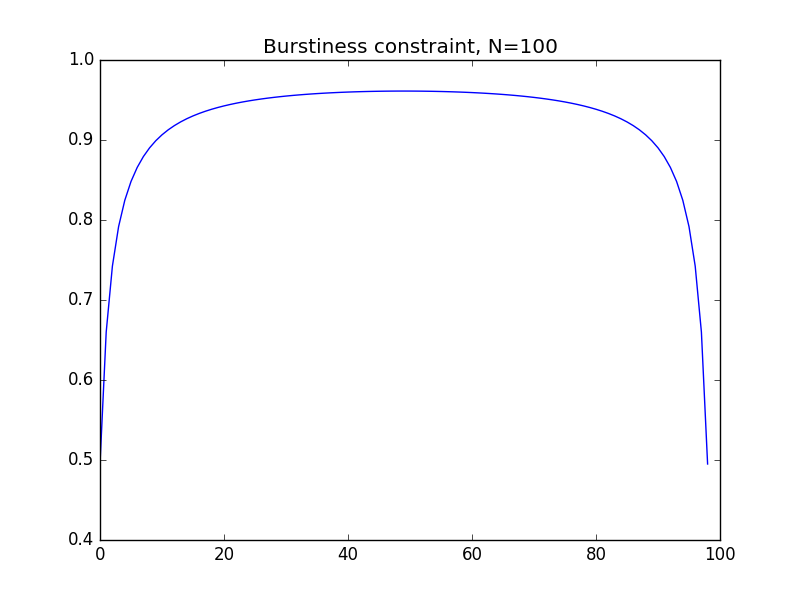
\includegraphics[scale=0.4]{\lpath/img/bp}
		\caption{This plot represent the series that constraints the predictive distribution for the burstiness effect in exchangeable graph for N=100 (100 nodes)}.
		\label{fig:bp}
	\end{figure}



\paragraph{Case of linear predictive distribution}~\\

A typical form of the predictive distribution $\p(y_{ij}=1 | d_i^{N,n})$ is a linear function of the sufficient statistics of the observations (see \ref{prop:diaconis}). We now study the burstiness effect in this case with regards to theorem \ref{th:burst_exch}.

We suppose that the predictive distribution has a linear form such that:

\begin{equation*}
p(y_{ij}=1 | d_i^{N,n}) = an+b
\end{equation*}  
Where $n$ is a positive integer and $a$ and $b$ two positive real numbers. From theorem \ref{th:burst_exch} one has the following condition in order to satisfy the global preferential attachment:

\begin{equation} \label{eq:polynom}
\frac{-an^2 -3an +a(N-1)-b(N+1)}{(n+2)(N-n)} > 0 
\end{equation}
The denominator of this equation strictly positive for $n \in [0, N-1]$. The condition depends then on the sign of the numerator. This polynomial of degree 2 admits 2 roots denoted $n_-$ and $n_+$ given by:
\begin{align*}
n_+ &= \frac{-3a + \sqrt{a(4N(a-b)+5a-4b)}}{2a} \\
n_- &= \frac{-3a - \sqrt{a(4N(a-b)+5a-4b)}}{2a} \\
\end{align*}

If we study the polynomial on the support of the real numbers, we can see that it is negative when $n$ tends to $+\infty$ and $-\infty$. Thus it takes positive values between the roots if they exists. The condition of existence is that the positivity of the roots:
\begin{equation*}
a(4N(a-b)+5a-4b) > 0 \iff b < a \frac{4N+5}{4N+4}
\end{equation*}

Furthermore, only one roots can be positive under the following constraint:
\begin{align*}
\sqrt{a(4N(a-b)+5a-4b)} > 3a \iff a\frac{N-1}{N+1} > b
\end{align*}

If such constraint is satisfied, the polynomial admits positive values for $n \in [0, n_+]$. This development shows that for certain form of the predictive distribution, the burstiness property can not be satisfied for all integers $n$. However a bursty phenomenon can exists on an interval $[0, n_+]$ whose upper bound is determined by the hyperparameters of the model.

We now study the local preferential attachments by formulating a second theorem that enable link from the definition to the predictive distribution. We will show that both theorem are related in a simple and natural way.

\begin{theorem}[Burstiness to Local Preferential Attachment] \label{th:burst_local}
    Let $\M_g$ be a network model of a jointly exchangeable graph $G(V,E)$. Let $N^c$ and $N^r$ be two integers such that the former is the number of nodes in a block $c \in \{0,.., K-1\}$, and the second the number of nodes not being in $c$, such that $N^c+N^r = N$. A local degree distribution $p(d_{i,c}=n)$ for any node $i$ in $c$ is bursty iif:
	
\begin{equation}
\Delta_n\   p(y_{ij}=1 | d_{i,c}^{N^c,n}) \frac{\sum_{r=0}^{N^r}\dbinom{N}{n+1+r} p(d_{ir}^{N^r,r})}{\sum_{r=0}^{N^r} \dbinom{N}{n+r} p(d_{ir}^{N^r,r}) } > 0
\end{equation}
	
\end{theorem}

\begin{proof}
The exchangeable graph $G(V,E)$ contains $|V|=N$ nodes. Thus in the context of the local preferential attachment we consider the degree of a node $i$ belonging to the block $c$ containing $N^c$ nodes. The degree of this node within this block is denoted by $d_{i,c}$ and the  number of node out of the block $c$ is equal to $N^r = N - N_c$. We can write the distribution of the degree inside that block by marginalizing the possible edges between node $i$ and the nodes that are not in $c$. We have:
\begin{equation*}
p(d_{ic}=n) = \sum_{r=0}^{N^r} p(d_{ic}=n,d_{ir}=r)
\end{equation*}
From exchangeable assumptions, it follows:

\begin{equation*}
p(d_{ic}=n) = \sum_{r=0}^{N^r} \dbinom{N}{n+r} p(d_{ic}^{N^c, n},d_{ir}^{N^r, r})
\end{equation*}

Under the assumptions that each local random parameters are i.i.d, we can separate the joint distribution: ( \textcolor{red}{on peut ouvrir la distribution avec les F et les Phi, pour voir que ca marche pour IMMSB EDIT: je pense que c'est en fait vrai pour ILFM aussi, le point clé etant que les poid $\phi_{kk}$ sont indépendement distribue ce qui fait que l'on peut séparer les partie correspondantes a chaque block.)}: 

\begin{align*}
p(d_{ic}=n) &= \sum_{r=0}^{N^r} \dbinom{N}{n+r} p(d_{ic}^{N^c, n}) p(d_{ir}^{N^r, r}) \\
 &=  p(d_{ic}^{N^c, n})\sum_{r=0}^{N^r}   \dbinom{N}{n+r} p(d_{ir}^{N^r, r})
\end{align*}

Finally by applying the burstiness properties as in proof \ref{proof:glob}, and product rule we can formulate the burstiness in function of the predictive distribution:

\begin{equation} \label{eq:29}
b_n =  p(y_{ij}=1 | d_{i,c}^{N^c,n}) \frac{\sum_{r=0}^{N^r}\dbinom{N}{n+1+r} p(d_{ir}^{N^r,r})}{\sum_{r=0}^{N^r} \dbinom{N}{n+r} p(d_{ir}^{N^r,r}) }
\end{equation}

\end{proof}

\textcolor{red}{Open Probem:  Je n'ai pas encore réussi à solver le ratio ci-dessus permettant de conclure sur le local bursty}


We can see that in the case where $N^r=0$ equation \eqref{eq:29} reduce to:
\begin{align*}
b_n &= p(y_{ij}=1 | d_{i,c}^{N^c,n}) \frac{\dbinom{N}{n+1}}{ \dbinom{N}{n} } \\
 &=  p(y_{ij}=1 | d_{i,c}^{N^c,n}) \frac{N-n}{n=1}
\end{align*}

And in this case $N^c=N$. This show that the results of theorem \ref{th:burst_exch} and \ref{th:burst_local} are equivalent in this case which is sounds since $N^r=0$ means that we consider link inside only one block, and so it is like evaluating the global preferential attachment.
%\begin{corollary}
%	A degree distribution  $p(d_i=n)$ of any node $i$ in a jointly exchangeable graph $G(V,E)$ such that it admits a predictive distribution of the form $\p(y_{ij}=1 | d_i^{N,n}) = an+b$, is bursty iff:
%Polynome solution, constraint on the positive roots, a, b > ...
%\end{corollary}

We now apply the previous results to characterize the preferential attachments effect in social networks.


\begin{proposition}
    The IMMSB model satisfies the local preferential attachment property in the generative version $\M_g$. \textcolor{red}{Pour conclure et raffiner la proposition, nous devons nous entendre sur les theorem V.1 et V.2 ( But theorem V.1 doesn't account for simulation that are always bursty with regards to the degree distribution.)}
\end{proposition}

\begin{proof}
In the generative IMMSB model, one can write in the general case the predictive distribution conditioned by $d_i^{N,n}$ has follows:

\begin{equation} 
p(y_{ij} = 1 | d_i^{N,n}, \mathcal{M}_g) = \int_{\Theta} p(y_{ij}=1|\Theta) \frac{p(d_i^{N,n} | \Theta)}{p(d_i^{N,n})} p(\Theta) d\Theta \nonumber
\end{equation}

Recall that in IMMSB the interaction $y_{ij}$ between two nodes $i$ and $j$ depends on their respective block assignments, and consequently, two nodes belongs to the same block $c$ if they took the same assignments (assignments are indicated in the variable $z$ drawing from the latent features in the generative process.).

In the context of the local preferential attachment property we consider only the relation inside this block $c$ and the predictive distribution is given by:

\begin{align*} \label{eq:sum}
&p(y_{ij} = 1 | d_{ic}^{N^c,n}, \mathcal{M}_g)  \\
&=  \frac{ \int_{\phi_{c}} p(y_{ij}=1|\phi_{c}) p(d_{ic}^{N,n} | \phi_{c}) p(\phi_{c}) d\phi_{c}}{\int_{\phi_{c}} \p(d_{ic}^{N^c,n} | \phi_{c}))       p(\phi_{c}) d\phi_{c}}   \\
&= \frac{\int_{\phi_c} \phi_c^{n+1}(1-\phi_c)^{N^c-n} \phi_c^{\lambda_1-1} (1-\phi_c)^{\lambda_0-1} d\phi_{c}}{\int_{\phi_c} \phi_c^{n}(1-\phi_c)^{N^c-n} \phi_c^{\lambda_1-1} (1-\phi_c)^{\lambda_0-1} d\phi_{c}} \\
&= \frac{ \text{B}(n+1+\lambda_1, N^c-n+\lambda_0) }{\text{B}(n+\lambda_1, N^c-n+\lambda_0)} \\
&= \frac{n+\lambda_1}{N^c + \lambda_1 +\lambda_0}
\end{align*}

where $\text{B}()$ is the beta function. Given the last equation it's obvious that the  predictive likelihood is linear with $n$.

    \paragraph{\textcolor{red}{Theorem \ref{th:burst_exch} Framework }}~\\

In particular,  let's now suppose that the predictive distribution takes this specific linear according to parameters :
\begin{equation*}
p(y_{ij}=1 | d_i^{N,n}) = \frac{n+\lambda_1}{N+\lambda_1+\lambda_0}
\end{equation*}
    This is equivalent to solving the polynomial \eqref{eq:polynom} for $a=1$ and $b=\lambda_1$. In such a case, the burstiness effect will be present in the subset $n \in \{0, n_+\}$ iff the following holds:
\begin{equation*}
\lambda_1 < \frac{N-1}{N+1}
\end{equation*}

    \paragraph{\textcolor{red}{Theorem \ref{th:burst_local} Framework }}~\\

    $\frac{\sum_{r=0}^{N^r}\dbinom{N}{n+1+r} p(d_{ir}^{N^r,r})}{\sum_{r=0}^{N^r} \dbinom{N}{n+r} p(d_{ir}^{N^r,r})}$  \textcolor{red}{ ? }

\end{proof}

\begin{proposition}
    The ILFM model does not satisfy the local preferential attachments in the generative model $\M_g$. \textcolor{red}{ meme question qu'audessus pour conclure cette proposition}
\end{proposition}

\begin{proof}
As for IMMSB proof, we only consider the relations  that occur inside block $c=\{k,k\}$, thus we note $N^c$ the total number of nodes being in the block $c$. In ILFM being in the block $c$ means that we evaluate the predictive distribution by only considering the column $c$ of the feature matrix. We can interpret this operation as looking the connections pattern when only the contribution of the feature $c$ is at work. One can write the predictive distribution inside this block as follows:

\begin{align*}
&\p(y_{ij}=1 | d_{ic}^{N^c,n}, \M_g)  \\
&=  \frac{ \int_{\phi_{c}} p(y_{ij}=1|\phi_{c}) p(d_{ic}^{N,n} | \phi_{c}) p(\phi_{c}) d\phi_{c}}{\int_{\phi_{c}} \p(d_{ic}^{N^c,n} | \phi_{c}))       p(\phi_{c}) d\phi_{c}} \\
&= \frac{ \int_{\phi_{c}} \sigma(\phi_c) \sigma(\phi_c)^n (1-\sigma(\phi_c))^{N^c-n}     p(\phi_{c}) d\phi_{c}}{\int_{\phi_{c}}  \sigma(\phi_c)^n (1-\sigma(\phi_c))^{N^c-n}      p(\phi_{c}) d\phi_{c}} \\
&= \frac{ \int_{\phi_{c}} \sigma(\phi_c) \sigma(\phi_c)^n \sigma(-\phi_c)^{N^c-n}     p(\phi_{c}) d\phi_{c}}{\int_{\phi_{c}}  \sigma(\phi_c)^n \sigma(-\phi_c)^{N^c-n}      p(\phi_{c}) d\phi_{c}} \\
&= \frac{ \int_{\phi_{c}} \sigma(\phi_c) (\frac{\sigma(\phi_c)}{\sigma(-\phi_c)})^n \sigma(-\phi_c)^{N^c}     p(\phi_{c}) d\phi_{c}}{\int_{\phi_{c}}  (\frac{\sigma(\phi_c)}{\sigma(-\phi_c)})^n \sigma(-\phi_c)^{N^c}     p(\phi_{c}) d\phi_{c}} \\
&= \frac{ \int_{\phi_{c}} \frac{\exp(n\phi)}{1+\exp(-\phi)} \frac{\exp(-N\phi)}{(1+\exp(-\phi))^{N^c}}  p(\phi_{c}) d\phi_{c}}{\int_{\phi_{c}}  \exp(n\phi) \frac{\exp(-N\phi)}{(1+\exp(-\phi))^{N^c}}   p(\phi_{c}) d\phi_{c}} \\
&= \frac{ \int_{\phi_{c}} \exp(\phi(n-N)) \sigma(\phi)^{N+1} p(\phi_{c}) d\phi_{c}}{\int_{\phi_{c}} \exp(\phi(n-N)) \sigma(\phi)^{N} p(\phi_{c}) d\phi_{c}} \\
\end{align*}

\begin{equation}
\int_{\phi_{c}} \exp(\phi(n-N)) \sigma(\phi)^{N+1} p(\phi_{c}) d\phi_{c} \ ?
\end{equation}


With $\sigma(\phi) = \frac{1}{1+\exp(-\phi)}$ and $\p(\phi) = \mathcal{N}(0, \sigma_w)$.



\textcolor{red}{not ended yet...same issue than the local case for IMMSB for the choice of the theorem.}
\end{proof}

We now turn to the mode $\M_e$. It is important to note here the fact that the probability $\pr(y_{ij}=1 \mid d_i \ge n, \M_e)$ increases with $n$ is equivalent to the fact that the probability $\pr(d_{i} \ge n+1 \mid d_i \ge n, \M_e)$ increases with $n$. Indeed:


\begin{align}
&\pr(d_{i} \ge n+1 \mid d_i \ge n, \M_e) \nonumber \\
&= 1 - \prod_{j \notin \mathcal{V}(i)} P(y_{ij} = 0 \mid d_i \ge n, \M_e) \nonumber \\
&= 1 - \prod_{j \notin \mathcal{V}(i)} (1 - P(y_{ij} = 1 \mid d_i \ge n, \M_e)) \nonumber
\end{align}


Hence $\pr(d_{i} \ge n+1 \mid d_i \ge n, \M_e)$ and $P(y_{ij} = 1 \mid d_i \ge n, \M_e)$ vary in the same direction. The same development holds for $\pr(y_{ij}=1 \mid d_{i,c} \ge n, \M_e)$. The above definitions, characterizing probabilistic link models in the mode $\M_e$ according to burstiness in social networks, are thus directly related to the general definition of burstiness given in Definition~\ref{def:burst}.


\begin{proposition}
	The ILFM and IMMSB models do not satisfy the global and local preferential attachments in the mode $\M_e$.
\end{proposition}

The proof of this statement is trivially true in the sens that given $\mat{F}$ and $\mat{\Theta}$, the likelihood is fully determined and hence do not depend on new links being generated. More precisely one has:
\begin{align*}
\p(y_{ij}=1| d_i \ge n, \M_e) &= \p(y_{ij}=1| \M_e)\\
&= \mat{\hat{f}}_{i} \mat{\hat{\Phi}} \mat{\hat{f}}_j^\top
\end{align*}
The predictive likelihood does not depend on $n$ and hence the burstiness is not satisfied. The same development holds for the local preferential attachment by indexing variables by the related block $c$.

One can note that, despite this result, the inference procedure of the posterior distribution will be likely to produce latent features that fit  the burstiness present in the data (if present) as reported in section \ref{sec:experiments}. This is particularly visible on the predictive likelihood for IMMSB which take the following form (see details in appendix \ref{sec:append}):
\begin{equation*} \label{eq:ppp}
p(y_{ij}=1 | \M_e)\propto \sum_{kk'} \frac{M_{(kk')1} + \lambda_1}{M_{(kk')\bm{.}} + \lambda_0 + \lambda_1}  (N_{ik} + \alpha\beta_k ) (N_{jk} + \alpha\beta_k)
\end{equation*}   
One can see that the features that are associated with the weights that cumulate number of observed links will be more likely to generate new links. In the case of ILFM the mixing between feature and weight is less clear since the non-conjugacy produce no close relation between the posterior and the sufficient statistics of the data (ie the degrees count). Nevertheless, the predictive analysis in section \ref{sec:experiments} shows that IMMSB outperform ILFM on bursty networks.

\begin{proposition} \label{prop:diaconis}
    ILFM model satisfy the burstiness effect for $n<n_+$ such that $n_+ \sim \sqrt{N}$  if $N>>0$ \\
    IMMSB model satisfy the burstiness effect for feature $k$, iif $n<n_+$ and $\alpha_k<\frac{N-1}{N+1}$ such that $n_+ \sim \sqrt{N(1-\lambda_1)}$ if $N(1-\lambda_1)>>0$ 
\end{proposition}

\begin{proof}
The Diaconis-Ilvisaker theorem \cite{diaconis1979conjugate} state \emph{'subject to regularity conditions, the conjugate priors typically used satisfy, and are characterized by, a  similar relation of posterior linearity'}:
\begin{equation}
\E_\Theta[\E_{X|\Theta}[X\mid \Theta] \mid X=x] = ax+b \quad \text{for} \quad x=0,1,2,... \nonumber
\end{equation}

Especially, the Dirichlet Process and the Indian Buffet Process, as prior for the latent features, are typically build on the suitable conjugate distribution, respectively a Dirichlet-Multinomial and a Beta-Bernoulli. Furthermore, this claim is highlighted by the Gibbs update the characterize their predictive distribution of feature and corroborate the feature burstiness effect:
\begin{align*} 
&\p(f_{ik} = 1 | F^{-ik}) = \frac{m_k^{-ik}}{N} \qquad \hspace{20pt} \text{ILFM feature update} \nonumber \\
&\p(f_{ik} = 1 | F^{-ik}) = \frac{n_{ik}^{-z_{ij}}+\alpha_k}{N+\alpha_.} \qquad \text{IMMSB feature update} \nonumber \\
\end{align*}

Where the $m_k^{-ik}$ described the number of elements that have the $k$-iem feature active except for element $i$, similarly $n_{ik}^{-z_{ij}}$ represents the number of times that $i$ was assigned to $k$ except for relation $(ij)$ (block membership are jointly sampled in MMSB).

By applying theorem \ref{th:burst_exch} for linear predictive distribution, we showed show that the burstiness is true until $n_+$ if the following polynomial admit a positive root:
\begin{equation*}
	 an^2 + 3an - a(N-1) + b(N+1) = 0
\end{equation*}

    In the case of ILFM and IMMSB, it is equivalent to solve the polynomial with $a=1$, $b=0$ for ILFM and $a=1$, $b=\alpha_k$ for IMMSB. The positive root arise in this case if $b < \frac{N-1}{N+1}$, which determines $n_+$. Thus for the ILFM, the root is only positive while for IMMSB, the positive root arise if $\alpha_k < \frac{N-1}{N+1}$. Moreover, when the number of nodes increase such that $N >> 0$, the born become $n_+ \sim \sqrt{N}$. The asymptotic born is the same for IMMSB if $\alpha_k << 1$.
\end{proof}

This proposition suggest that HDP and IBP are admissible priors in order to satisfy a burstiness effect on the latent features until a reasonable born. This born is asymptotically  (with a mild condition on IMMSB), the square root of the number of nodes. Note that the constraint that we find for the condition over the hyperparameters of the truncated Dirichlet (for IMMSB), directly traduce the well know fact that the more the parameters of a Dirichlet distribution are small the more the sample will be sparse. Or equivalently, the distribution will be concentrated on the corners of its simplex.

\subsection{Empirical Illustration}

We illustrate the burstiness results by generating 3 random networks for each of both models. We report it in figure \ref{fig:gen_burst}. We use the 3 same settings for IMMSB  than those in the previous section. For ILFM  we use the following 3 settings: (column 1:$\alpha=1,  \lambda_1=\lambda_2=1$ , column 2:$\alpha=0.1, \lambda_1=\lambda_2=1$, column 3: $\alpha=1, \lambda_1=\lambda_2=10$) and we fix $\sigma_w=1$ and again $N=1000$.

Each row of the two sets of figures represents the three following measures who corresponds respectively to the global preferential attachment, the local preferential attachment and the feature burstiness:
\begin{itemize}
    \item First row: we measure the overall degree distributions; We report the average and standard deviation of the degree distribution in a linear scale for each generated network.
    \item Second row: we measure the local degree distribution on a log-log scale:
        \begin{itemize}
            \item for IMMSB, each network has an associated membership tensor $Z$, that indicates the membership of nodes for each  interactions. In order to draw the local degree distribution for a block $c$, we reduce the adjacency matrix in order to retain only the links that occurs inside a block $c$. The local degree distribution is thus computed on the reduce adjacency matrix $Y_c = Y \otimes (Z_i^c \times Z_j^c)$ where $\otimes$ is the hadamard product and $\times$ the outer product. $Z_i^c$ is the membership matrix of a nodes $i$ such that $Z_{ik}^c=0$ if $k\neq c$ (links that occurs outside $c$ will be ignored).
            \item for ILFM, each node is associated with a fix feature vector; the local degree distribution for the block $c$ is obtain by taking only the contribution of the features $c$ on the adjacency matrix. Thus, the local degree degree distribution is computed on the reduce adjacency matrix $Y_c = Y \otimes (F_{.c}\times F_{.c})$. 
        \end{itemize}
    \item Third row measure the distribution of the block membership, which directly reflect the feature burstiness. Hence for IMMSB, for a feature $k$, we measure $\sum_{ij} \mathds{1}(Z_{i\rightarrow j} = k, Z_{i\leftarrow j} = k)$ which indicates the number of nodes who were associated to the block $k$. For ILFM the number of nodes associated to a block $k$ is simply $\sum_n F_{nk}$.
\end{itemize}


% not sure it use significantly usefull, because p-value are either 0 or 1 ...
%We provide in annexe (\textcolor{red}{not yet included}),  an goodness of fit for all local degrees distribution that we plotted, in order to quantify the power law hypothesis on the empirical degree distributions. The number of feature is typically too small to evaluate an significant goodness of fit. The protocol is described in section \ref{sec:experiments-busrt}. 

The simulation shows us the following facts about the properties of the models:
\begin{itemize}
	\item For both model the global degree distribution don't exhibit a bursty phenomenon,
	\item The local degree distribution show that IMMSB exhibit a bursty phenomenon which is not the case for ILFM,
	\item Both models exhibits a bursty phenomenon on the feature distribution. This distributions for ILFM has a long tail for all of the 3 settings while for IMMSB, the tail shape is more or less long depending of the $\alpha$ and $\gamma$ parameters.
\end{itemize}

For the case of the global preferential attachment we have no formal proof for the non-compliance of the models, due the non closed form of the evidence in both models, due to the admixture design \textcolor{red}{ref ((Multiple Hypergeometric Functions: Probabilistic Interpretations and Statistical Uses
James M. Dickey )) ce papier est cite dans LDA pour justifier l'inference approxime, mais je n'arrive pas a trouver ca papier !!!}. However, as reported simulations (figure \ref{fig:gen_burst}), we see that the empirical distributions of the overall degrees are clearly non bursty.


\begin{figure*}[ht]
	\centering IMMSB\\
	\minipage{0.27\textwidth}
	\includegraphics[scale=0.27]{\lpath/img/M_g_peaks/figure_1}
	\endminipage
		\minipage{0.27\textwidth}
	\includegraphics[scale=0.27]{\lpath/img/M_g_power_law/figure_1}
	\endminipage
	\minipage{0.27\textwidth}
	\includegraphics[scale=0.27]{\lpath/img/M_g_regular/figure_1}
	\endminipage
		\vspace{-0.29cm}
	\minipage{0.27\textwidth}
	\includegraphics[scale=0.27]{\lpath/img/M_g_peaks/figure_3}
	\endminipage
		\minipage{0.27\textwidth}
	\includegraphics[scale=0.27]{\lpath/img/M_g_power_law/figure_3} 
	\endminipage
	\minipage{0.27\textwidth}
	\includegraphics[scale=0.27]{\lpath/img/M_g_regular/figure_3}
	\endminipage
		\vspace{-0.28cm}
	\minipage{0.27\textwidth}
	\includegraphics[scale=0.27]{\lpath/img/M_g_peaks/figure_5}
	\endminipage
	\minipage{0.27\textwidth}
	\includegraphics[scale=0.27]{\lpath/img/M_g_power_law/figure_5} 
	\endminipage
	\minipage{0.27\textwidth}
	\includegraphics[scale=0.27]{\lpath/img/M_g_regular/figure_5}
	\endminipage

    \vspace{0.2cm}
	 ILFM

	\minipage{0.27\textwidth}
	\includegraphics[scale=0.27]{\lpath/img/ilfm/1/figure_1}
	\endminipage
		\minipage{0.27\textwidth}
	\includegraphics[scale=0.27]{\lpath/img/ilfm/2/figure_1}
	\endminipage
	\minipage{0.27\textwidth}
	\includegraphics[scale=0.27]{\lpath/img/ilfm/3/figure_1}
	\endminipage
		\vspace{-0.29cm}
	\minipage{0.27\textwidth}
	\includegraphics[scale=0.27]{\lpath/img/ilfm/1/figure_3}
	\endminipage
		\minipage{0.27\textwidth}
	\includegraphics[scale=0.27]{\lpath/img/ilfm/2/figure_3} 
	\endminipage
	\minipage{0.27\textwidth}
	\includegraphics[scale=0.27]{\lpath/img/ilfm/3/figure_3}
	\endminipage
		\vspace{-0.28cm}
	\minipage{0.27\textwidth}
	\includegraphics[scale=0.27]{\lpath/img/ilfm/1/figure_5}
	\endminipage
	\minipage{0.27\textwidth}
	\includegraphics[scale=0.27]{\lpath/img/ilfm/2/figure_5} 
	\endminipage
	\minipage{0.27\textwidth}
	\includegraphics[scale=0.27]{\lpath/img/ilfm/3/figure_5}
	\endminipage
    \caption{Generated Networks with IMMSB (top) and ILFM (bottom) for three different settings (same set than for figure \ref{fig:gen_blocks_mmsb}). The top rows measure the global preferential attachment through the overall degree distribution. The middle row measure the local preferential attachment through the local degree distribution. The last row measure the feature burstiness through the block membership distribution.}
	\label{fig:gen_burst}
\end{figure*}


\section{Feature Dynamic}
\label{sec:dynamic}

We defined the notion of latent features previously, where features is related to the membership of nodes in latent space.  The question that we ask here, is how the total number of latent features -- its dimension -- evolve with the size of the network ie its number of vertices.

%Hence one can have theintuition that if links are mostly created in a set of class (inner or outer), the shortest path between two random nodes is``proportional'' to the number of step needed to go through all classes $K$.

The dimension of the features in the ILFM is given through the Indian Buffet Process. Though, in its metaphor, each new customers $i$ draws Poisson$(\frac{\alpha}{i})$ new dishes. Thus the expectation of the dimension of the features is:

\begin{align*}
\E[K|\alpha, N] &=  \sum_{i=1}^N \frac{\alpha}{i} = \alpha H_n \\
&= \alpha(\log(n) + \gamma +O(1/N) ) \qquad  \text{for} \quad N >> 0
\end{align*}
Where $\gamma$ is the Euler-Mascheroni constant.\\

Similarly, in a case of IMMSB, the dimension of the classes is potentially infinite and evolves with the data through an Hierarchical Dirichlet Process (HDP) prior.

In the HDP, we have two step DP that form a so called Chinese Restaurant Franchise (CRF) where each restaurant has an infinite capacity, and in its metaphor one has:
\begin{itemize}
\item The CRF has a shared menu constituted of dishes that symbolize the classes.
\item the number of table in each restaurant, where restaurant symbolically correspond to nodes and tables represent a couple of classes $(k,k')$ where a node generate some links (and non links) with other nodes. 
\item the total number of dishes in the franchise, where each table is associated to a couple of dishes, (where dishes represent the classes).
\end{itemize}

By definition of a \(DP(\alpha)\), we know that for each new draw given
\(i\) previous draws, the probability to generate a new group is equal
to \(\frac{\alpha}{\alpha +i-1}\) independently of the number of previous
component created. Moreover in the CRF, each table is drawn from a DP while the classes for each tables are drawn from one another DP (shared in all the franchise). Thus we can express the expectation of the number of tables ($\E[T|N, \alpha_0]$) and classes ($\E[K|T, \gamma]$). We start by the first quantity, for an undirected graph of size $N >> 0$:

\begin{align*}
&\E[T|N, \alpha_0] = \sum_{j=1}^N\sum_{i=1}^{2N} \frac{\alpha_0}{\alpha_0 +i-1} \\
& \alpha_0 N (\Psi(\alpha_0+2N) - \Psi(\alpha_0))
\end{align*}
Given the properties of the $\Psi$ function, we the asymptotic behavior of $\E[T|N]$ is :

\begin{equation*} \label{eq:e_t}
\E[T|N, \alpha_0] \sim \alpha_0 N \log(\frac{2N}{\alpha_0}) \qquad \text{if} \quad N >> \alpha_0 >> 0
\end{equation*}

Similarly, for the expectation of the dimension of the classes, we have:

\begin{equation*}
\E[K|T, \gamma] = \sum_{i=1}^{T} \frac{\gamma}{\gamma +i-1} = \gamma (\Psi(\gamma+T) - \Psi(\gamma))
\end{equation*}

One can remark, from equation \eqref{eq:e_t}, that $\lim_{N\to\infty} \E[T|N] \to  \infty$. Thus the expected limit for the number of cluster by chaining the two DP is:

\begin{equation*}
\E[K] = \gamma \log(\frac{\alpha_0 N}{\gamma}\log(\frac{2N}{\alpha_0} )) \qquad \text{if} \quad N >> \gamma>>0
\end{equation*}

We conclude that the latent features grow logarithmically with the number of nodes.

We show the empirical evolution of the dimension of classes generated by the HDP that we reported in figure \ref{fig:gen_dyn}. 

\begin{figure}[h]
	\centering
	
	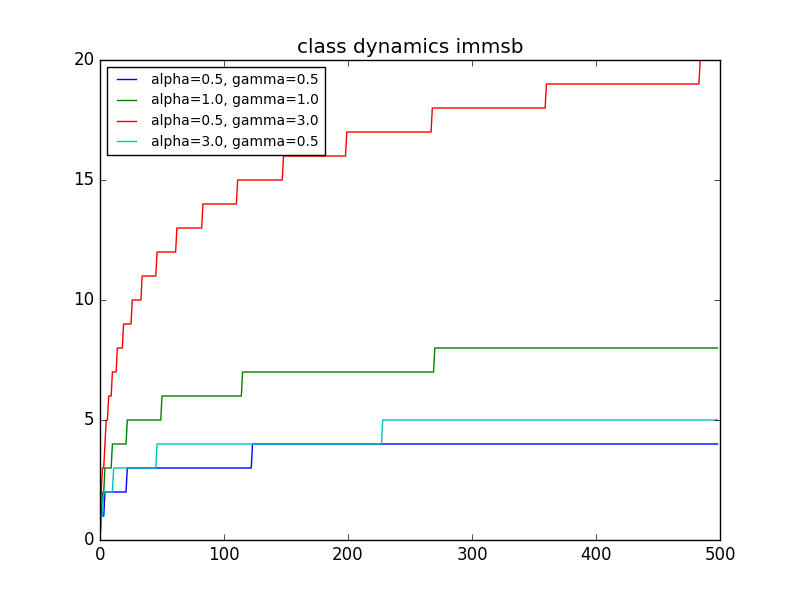
\includegraphics[scale=0.4]{\lpath/img/class_dynamics}
	%	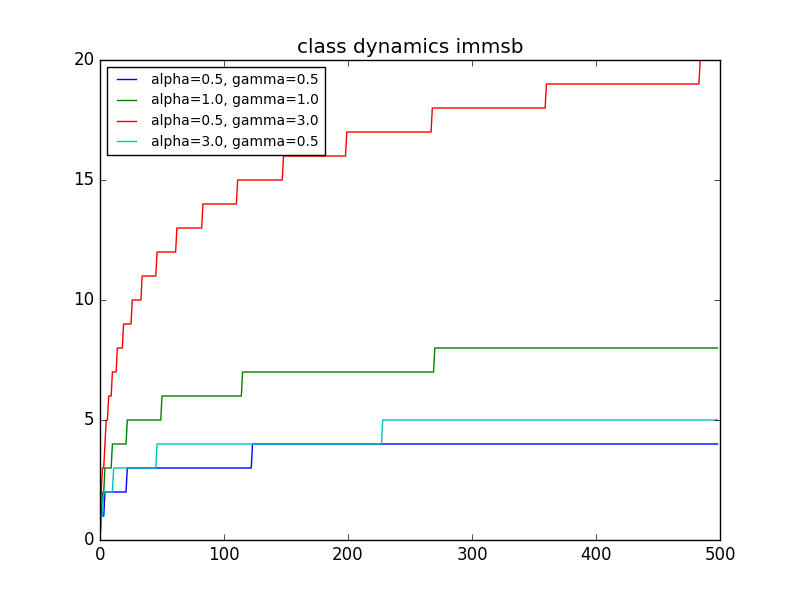
\includegraphics[width=3.2cm, height=3.7cm]{\lpath/img/class_dynamics}

	\caption{Each curve correspond to a different setting of hyperparameters for IMMSB. For each X-axis correspond the nomber of nodes, for which we generated a networks. The Y-axis is the number of latent features to which HDP converged. Those figure illustrate the logarithm shape of the evolution of number of feature $K$ with the number of nodes $N$ in the networks.}
	\label{fig:gen_dyn}
\end{figure}


\section{Sparsity}
\label{sec:sparsity}

The last property we study in this paper is the sparsity. Sparsity is the fact that most values in a dataset are empty. Whenever a feature space can be big, an object would end up with most of his features to be equal to zero. In networks, the sparsity is directly quantified by the density of the network which means that a few number of edges is actually observed compared to set of possible edges in the network proportional to $\dbinom{N}{2}$. An other typical example where sparsity appears, is in text collections, where a few words of the dictionary appears in each document.

%defnition of dense and sparse netwroks are given in Bayesian Models of Graphs, Arrays and Other Exchangeable Random Structures(Peter Orbanz and Daniel M. Roy) \\

%definition of exchangeability for networs first mention in this interesting paper: Modeling homophily and stochastic equivalence in symmetric relational data [Hoff]


For probabilistic models, the density for undirected networks of size $|V|=N$, is defined by the expectation of generating a link, which represents the average chance to observe a link between two nodes. Hence this quantity is, in the $M_g$ settings:
%\begin{equation}
%p(y_{ij}^{new}=1| |V|=N) =  \int_{\Theta} p(y_{ij}^{new}=1|\Theta) \frac{\sum_{n=0}^{\dbinom{N}{2}} p(d^N=n| \Theta)}{\int_{\Theta} \sum_{n=0}^{\dbinom{N}{2}} p(d^N=n | \Theta)) p(\Theta) d\Theta} p(\Theta) d\Theta
%\end{equation}
%Where  $p(d^N=n)$ is the probability of a random graph with $N$ vertices and having $n$ edges. Thus it refers to the density of the graph. We now define the set of  adjacency matrix $Y_r$ corresponding to the ensemble of graphs having $n$ edges (and $N$ vertices) $Y_r \in \{Y: d=n\}$. Because of the exchangeability of the models, each of those adjacency matrices have the same distribution under joint random permutation of rows and colomns, given $\Theta$, and the number of different graph that occurs are $\dbinom{N}{C(Y_r)}$, with $C(Y_r)$ is the number of nodes of $Y_r$ having a non empty degree:
%\begin{equation}
%p(y_{ij}^{new}=1| |V|=N) =  \int_{\Theta} p(y_{ij}^{new}=1|\Theta) \frac{\sum_{n=0}^{\dbinom{N}{2}} \sum_{Y_r \in \{Y: d=n\}}\dbinom{N}{C(Y_r)} p(Y_r| \Theta)}{\int_{\Theta} \sum_{n=0}^{\dbinom{N}{2}}  \sum_{Y_r \in \{Y: d=n\}}\dbinom{N}{C(Y_r)} p(Y_r | \Theta)) p(\Theta) d\Theta} p(\Theta) d\Theta
%\end{equation}


%Here, one can see that from excheangeability we can take out the sum over graph from the integral on the parameters. The density take though a similar form than equation  \eqref{eq:sum}. We have then that $\Delta_N p(y_{ij}^{new}=1| |V|=N) >0 $.

\begin{align*}
&p(y_{ij}^{new}=1| \mathcal{M}_g) = \int_{f_i} \int_{f_j} \int_{\Phi} p(f_i| \alpha ) p(f_j| \alpha)p(\Phi| \lambda) \\
&\times \sum_{k<k'} p(y_{ij} \mid \phi_{kk'})\ p(k\mid f_i)p(k'\mid f_j)df_i df_j d\Phi \\
&=  \sum_{k<k'} \int_{\Phi} \phi_{kk'} p(\Phi| \lambda) d\Phi \int_{f_i} f_{ik} p(f_i| \alpha )df_i \int_{f_j} f_{jk}  p(f_j| \alpha ) df_j \\
&= \sum_{k<k'} \E[B(\lambda_1, \lambda_0)] \E[Dir(\mat{\alpha} )]_k \E[Dir(\mat{\alpha})]_{k'} \\
&= \frac{\lambda_1}{\lambda_0+\lambda_1}\frac{\sum_{kk'} \alpha_k\alpha_k'}{(\sum_k \alpha_k)^2} = \epsilon
\end{align*}


We see that the density do not dependent of $N$, and thus the number of edge grows with $N^2$ since its expectation is  $\dbinom{N}{2} \epsilon$.

This result shows that the model generate dense networks because the model is misspecified. More precisely, this results can be generalize for all graph that have an assumption of exchangeability, and particularly this exchangeability assumptions is true for the two models we studied here, though less obvious for ILFM since IBP doesn't draw independent feature vector, but the nodes exchangeability is inherited from the features exchangeability of the IBP \cite{orbanz2015bayesian}. This strong result is a direct consequence of the Haldous-Houver representation theorem for exchangeable array which generalize the de Finetti theorem for exchangeable sequence \cite{orbanz2015bayesian}. 

\section{Prediction Evaluation}
\label{sec:experiments}

In previous sections, we shown theoretical results with empirical measures  on realization of networks using the generative property of the probabilistic models. In this section, we seek to explain the predictive performance on several datasets by examining their empirical properties and how well the models can capture them. This analysis provide also a study on a comparison of both models, IMMSB and ILFM. Particularly we will see that performance of those models really depend on the type of data we want to fit.

This section is organized as follows:  In first subsection we described our goodness of fit measure used to evaluate various degree distribution. In the second we present the synthetic and real dataset that we have used. In the third we present our prediction evaluation setting. In the last we report our results.

\subsection{A measures for the preferential attachment effect}

\label{sec:experiments-burst}
Preferential attachment leads to networks characterized by a degree distribution with heavy tail. A typical form of such law, often meet in data, is a a power law distribution. Comparison of the degree distribution with a linear function in the log-log scale  gives us a qualitative measure for the preferential attachment. However, for a better evaluation of the power law hypothesis on the degree distribution, we rely on a  goodness a fit based on a Kolmogorov-Smirnov (KS) test. We follow the protocol described in \cite{clauset2009power} which consists of the following steps:
\begin{itemize}
	\item Estimate the parameters $x_{min}$ and $\alpha$ of the power law model.
	\item Calculate the goodness of fit between synthetic datasets generated with the power law and the data. The resulting $p$-values gives an estimates of the  plausibility of the hypothesis for the data.
\end{itemize}

As mentioned in \cite{clauset2009power} high value of the $p$-value should be considered with caution for at least two reasons. First, there may be other distribution that match the data equally or better. Second, a small number of samples of the data may lead to high p-value and reflect the fact that is hard to rule out an hypothesis in such a case.

\subsection{Datasets}
In our experiments, we consider four artificial networks and two real networks.\\

\textit{Artificial networks}

The artificial networks have been generated with ANC-Generator \cite{largeron2015}. This generator has been chosen because it allows to build attributed graphs with  community structure faithfully following the known properties of real-world networks such as preferential attachment and homophily.
Moreover, by modifying the parameters, these properties can be weakened. Finally, ANC-Generator is available under the terms of the GNU Public License and the        parameters can be shared for experiments reproducibility.

Four artificial networks have been generated, each one corresponding to a configuration  regarding the properties of interest.
Table \ref{table:artificial_networks} summarizes these four configurations. We report the seed and parameters that we use those synthetic networks in appendix \ref{seed_dancer	}. Each generated networks correspond to a different combination where homophily and preferential attachment are more or less characterizing the underlying networks. For example...

\begin{table}[h] \label{table:artificial_networks}
	\caption{Artificial networks characteristic.}
	\begin{tabular}{lrrrr}
		\hline
		Networks   &  p-value    &  Modularity & Clustering coefff & density   \\
		\hline
		$Network1$    & 1 &0.59  & 0.06 & 0.007  \\
		$Network2$   & 1 &0.43  & 0.08 & 0.006\\
		$Network3$  & 0.52  &0.71  & 0.49 & 0.01 \\
		$Network4$   & 0.57  &0.68  & 0.61 & 0.06 \\
		\hline
	\end{tabular}
	\caption{Real networks characteristic}
	\begin{tabular}{lrrrr}
		\hline
		Networks    &  p-value    &  Modularity & Clustering coefff & density   \\
		\hline
		$fb\_uc$          & 1 & -  & 0.10 & 0.008 \\
		$manufacturing$   & 0.42 & -  & 0.59 & 0.24 \\
	\end{tabular}
\end{table}

\textit{Real networks}

We also used two real world networks for our experiments .
The first one \footnote{available at:} is built from an online community of 1899 students from the University of California. Each node corresponds to a user and a    directed edge represents a sent message.
The second one \footnote{available at:} is an internal email communication network between employees of a mid-sized manufacturing company. Each vertex is associated  to an employee and an oriented link represents like previously a sent email.

Table 1 summarizes some properties characteristics of these artificial and real datasets. The  p-value is computed as described in \ref{sec:experiments-burst } as a reference for the global preferential attachment effect. we also report the modularity on the a given (true) partition (by Dancer) of the networks, and the clustering coefficient.

\begin{figure}[h]
	\centering
	
	\minipage{0.25\textwidth}
	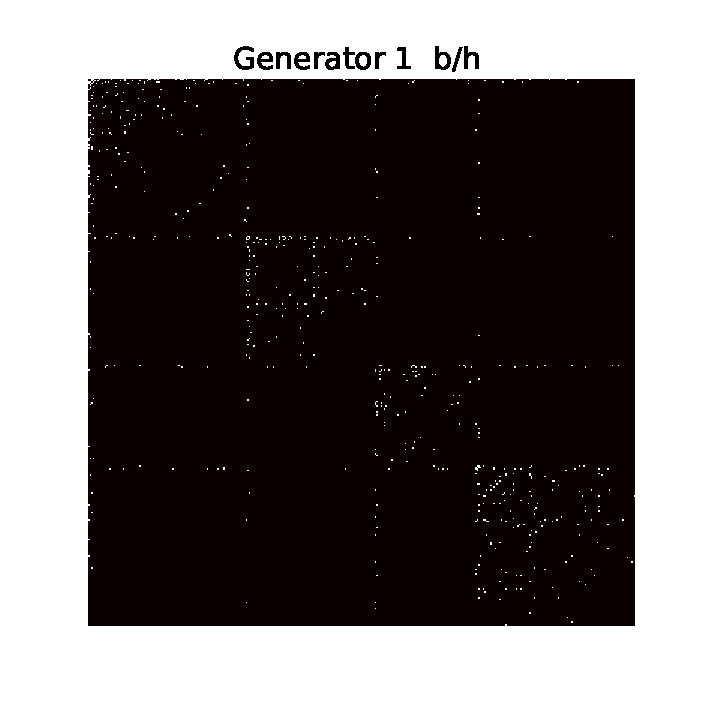
\includegraphics[scale=0.4]{\lpath/img/g1}
	\endminipage
	\minipage{0.25\textwidth}
	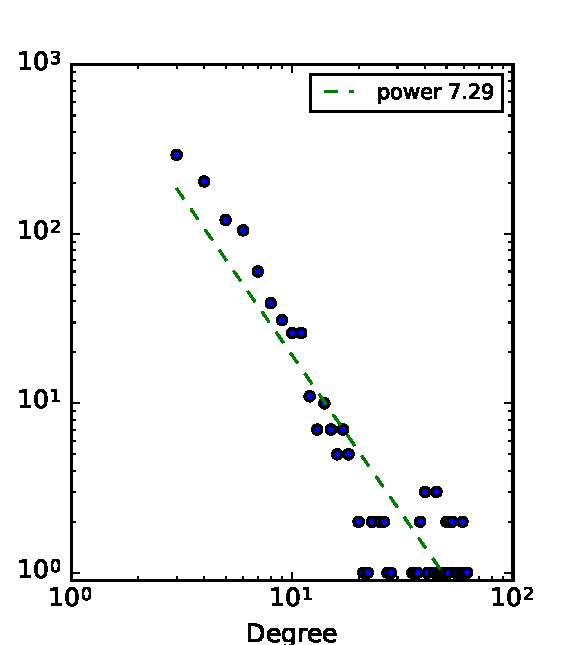
\includegraphics[scale=0.4]{\lpath/img/g1_d}
	\endminipage
	\vspace{-0.4cm}
	\minipage{0.25\textwidth}
	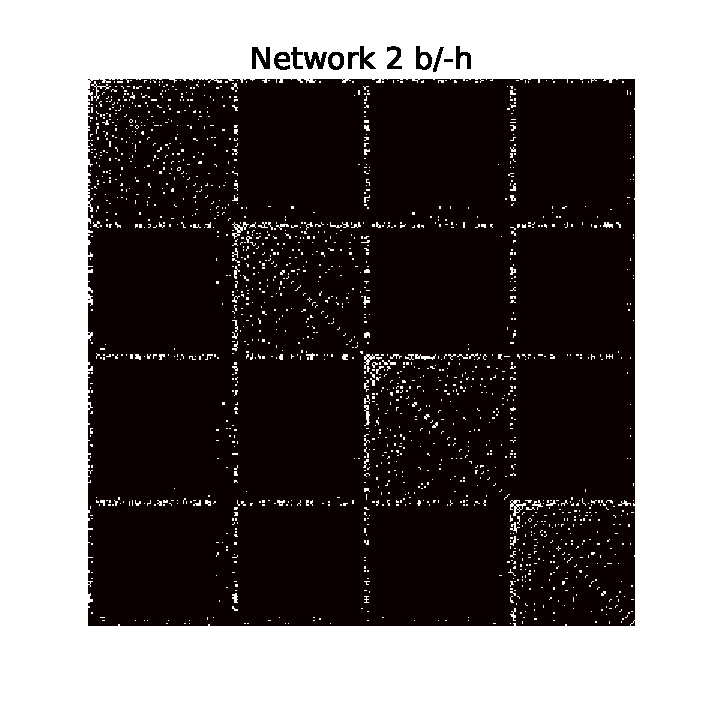
\includegraphics[scale=0.4]{\lpath/img/g2}
	\endminipage
	\minipage{0.25\textwidth}
	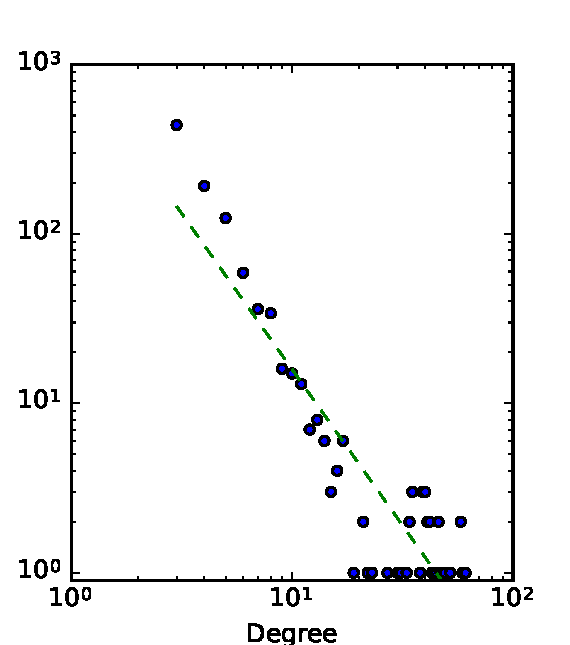
\includegraphics[scale=0.4]{\lpath/img/g2_d}
	\endminipage
	\vspace{-0.4cm}
	\minipage{0.25\textwidth}
	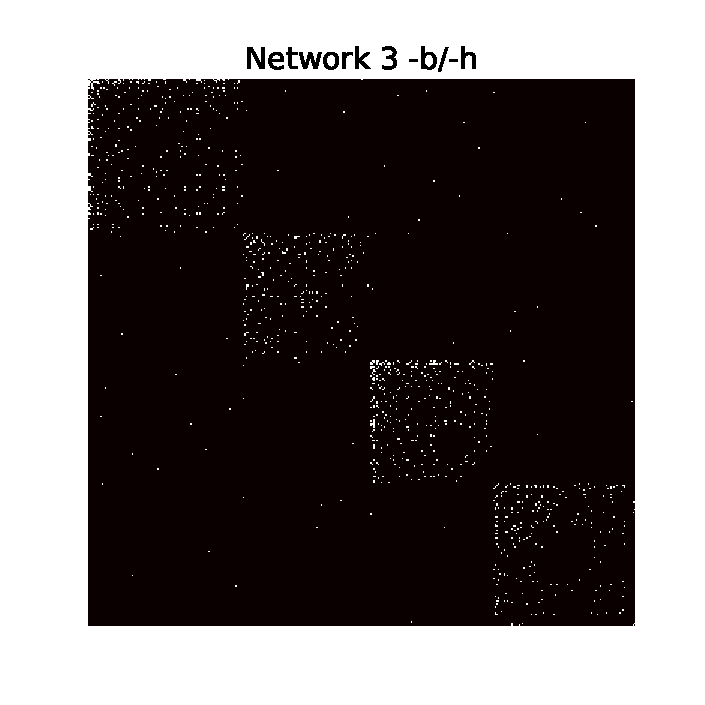
\includegraphics[scale=0.4]{\lpath/img/g3}
	\endminipage
	\minipage{0.25\textwidth}
	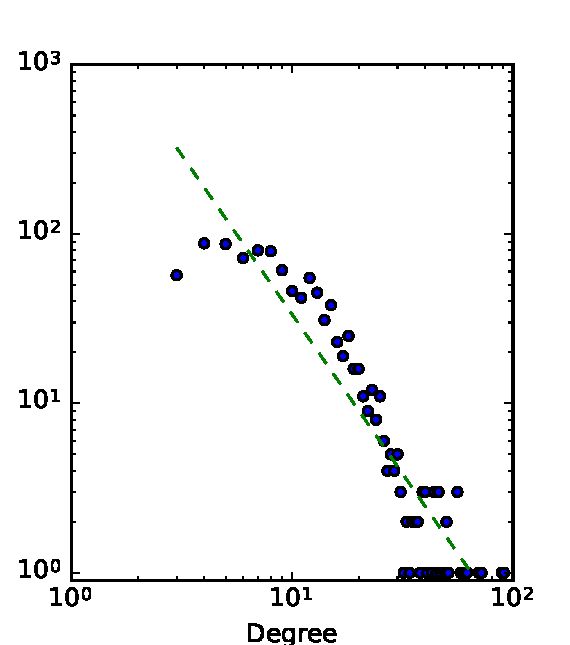
\includegraphics[scale=0.4]{\lpath/img/g3_d}
	\endminipage
	\vspace{-0.4cm}
	\minipage{0.25\textwidth}
	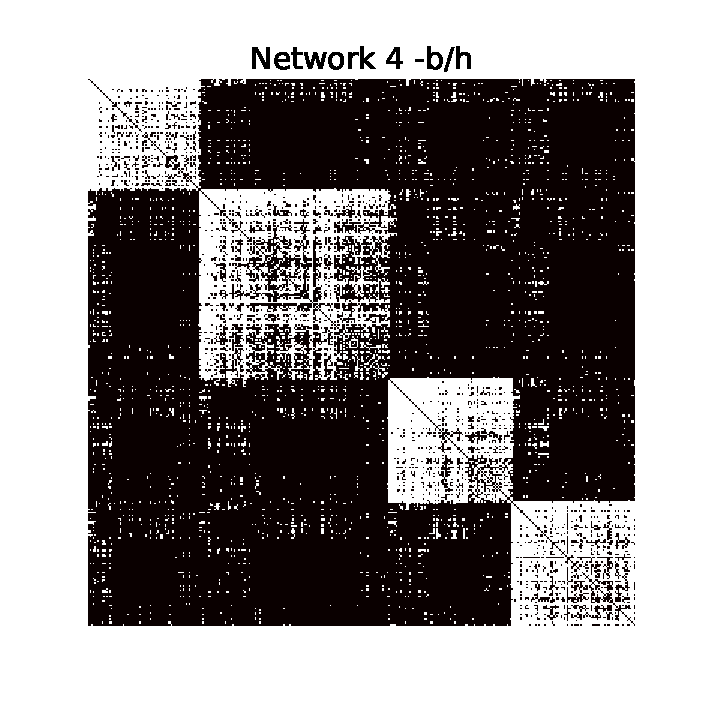
\includegraphics[scale=0.4]{\lpath/img/g4}
	\endminipage
	\minipage{0.25\textwidth}
	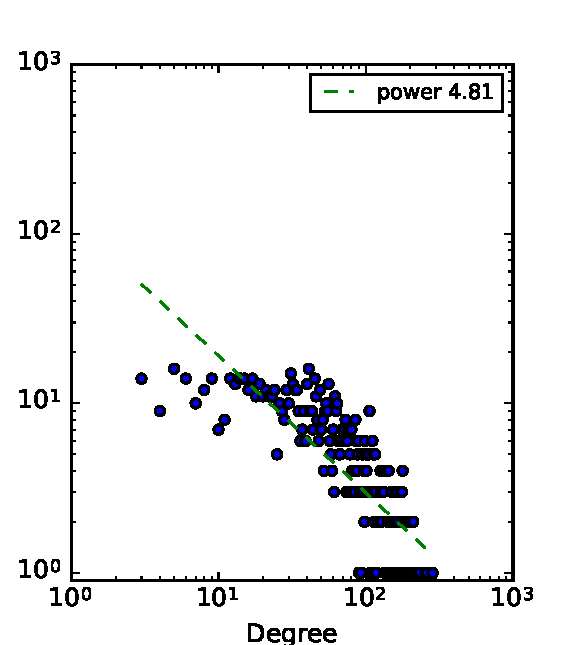
\includegraphics[scale=0.4]{\lpath/img/g4_d}
	\endminipage
	
	\caption{Left figures represent the adjacency matrices (left) for each of the 4 synthetic networks that we used for the prediction evaluation along their respective global degree distribution in the right plots.}
	\label{fig:synt_graph}
\end{figure}

\begin{figure}[h]
	\centering
	
	
	\minipage{0.25\textwidth}
	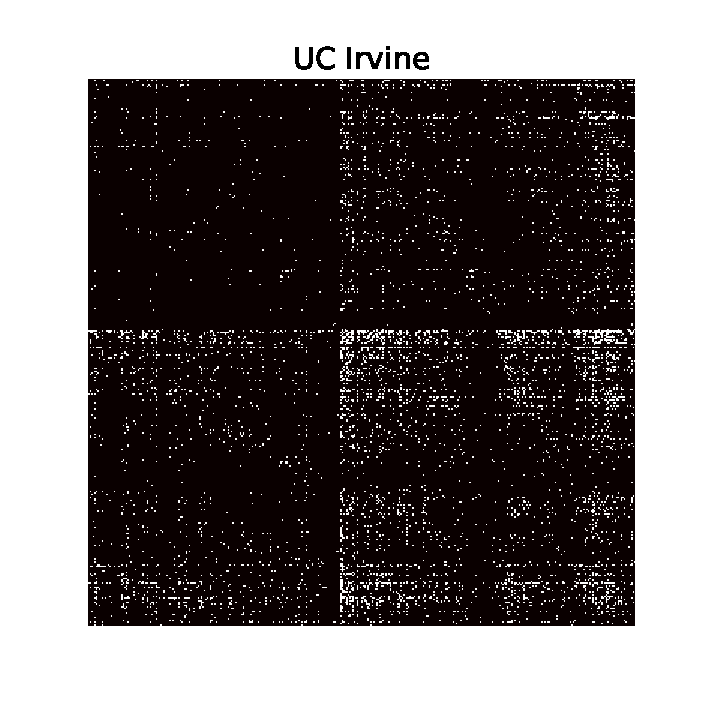
\includegraphics[scale=0.4]{\lpath/img/irvine}
	\endminipage
	\minipage{0.25\textwidth}
	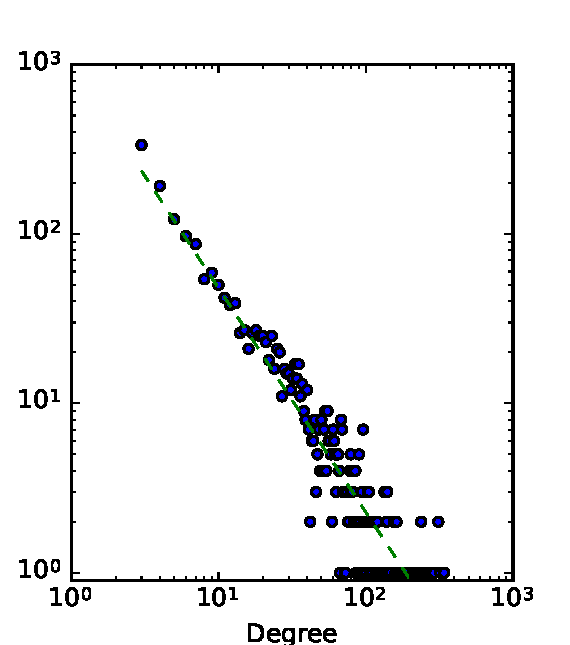
\includegraphics[scale=0.4]{\lpath/img/irvine_d}
	\endminipage
	\vspace{-0.4cm}
	\minipage{0.25\textwidth}
	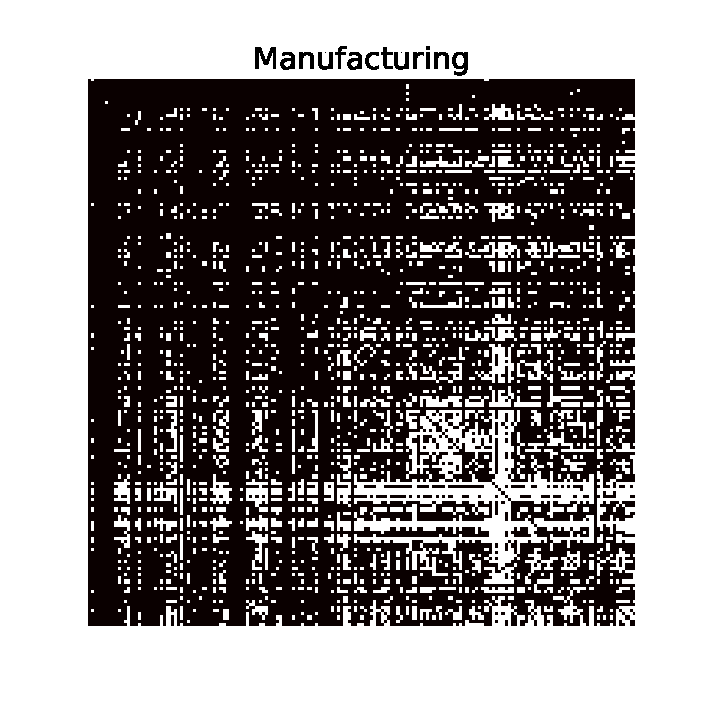
\includegraphics[scale=0.4]{\lpath/img/manufacturing}
	\endminipage
	\minipage{0.25\textwidth}
	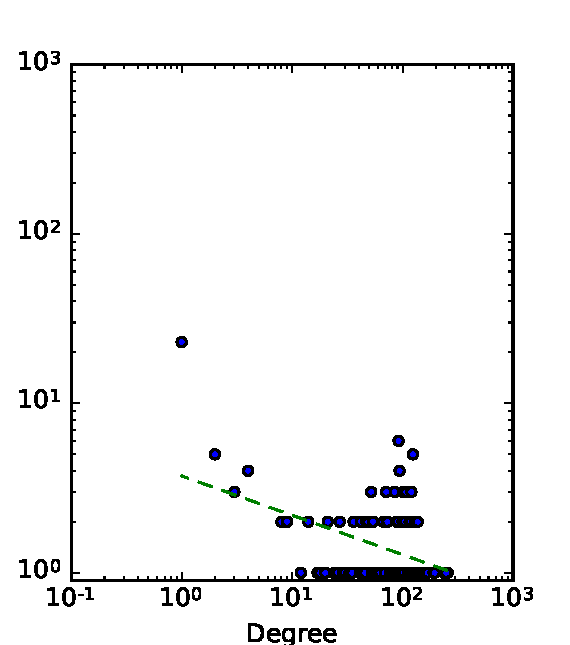
\includegraphics[scale=0.4]{\lpath/img/manufacturing_d}
	\endminipage
	\caption{Left figures represent the adjacency matrices (left) for each of the 2 real networks that we used for the prediction evaluation along their respective global degree distribution in the right plots.}
	\label{fig:real_graph}
\end{figure}



\subsection{Experimental Settings}
For each datasets described,  we run a MCMC inference consisting of 200 iterations to learn the posterior distribution of each the IMMSB model and ILFM, described in \ref{sec:models}. For IMMSB, concentration parameters of HDP were optimized following \cite{HDP} using vague gamma priors $\alpha_0 \sim \text{Gamma}(1,1)$ and       $\gamma \sim \text{Gamma}(1,1)$. The parameter for the matrix weights were fixed to $\lambda_0=\lambda_1=0.1$. For ILFM, the IBP hyper-parameter was fixed to   $\alpha=0.5$ and the weights hyper-parameter to $\sigma_w = 1$. Each experiences were averaged on 10 repetitions, and results were found to be stable regarding on the random  initialization and the stochastic optimization procedure. 
 

We evaluate the  prediction performance of the models by building a training set and a testing set from the original datasets. In order to achieve this, we build a random mask consisting of 20 percent of the size of the adjacency matrix. This mask is used a our testing set, while the 80 remaining percent are used as a training set.

The inference procedure was run under this settings in all of the 4 synthetic datasets and 2 real networks.

All our experimental platform is available online \footnote{https://github.com/dtrckd/pymake}. It is an ongoing development in order to provide a flexible way to design and run experiments and make data analysis.


\begin{figure}[h]
	\centering
	
	\minipage{0.25\textwidth}
	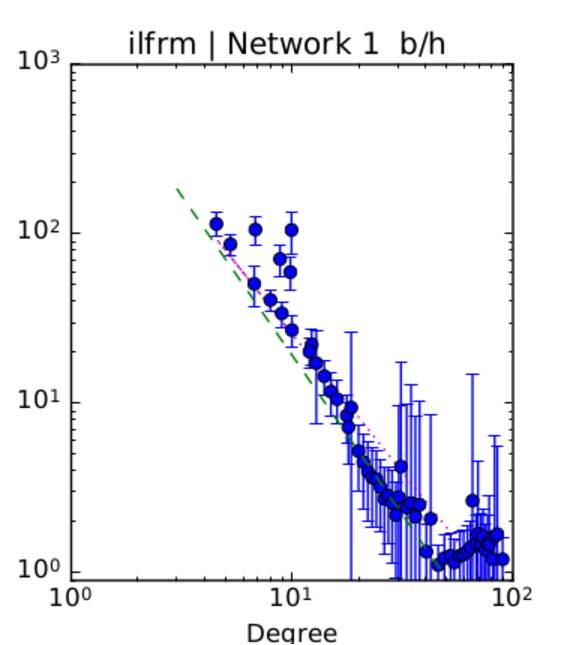
\includegraphics[scale=0.4]{\lpath/img/ilfrm_g1_d}
	\endminipage
	\minipage{0.25\textwidth}
	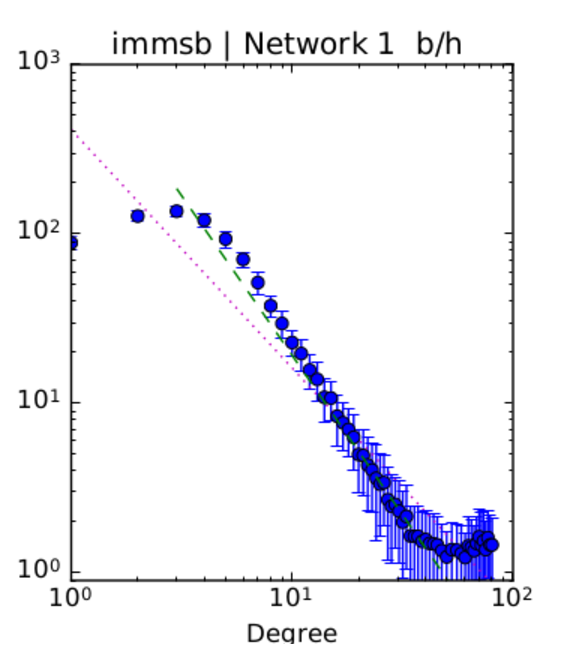
\includegraphics[scale=0.4]{\lpath/img/immsb_g1_d}
	\endminipage
	\vspace{-0.4cm}
	\minipage{0.25\textwidth}
	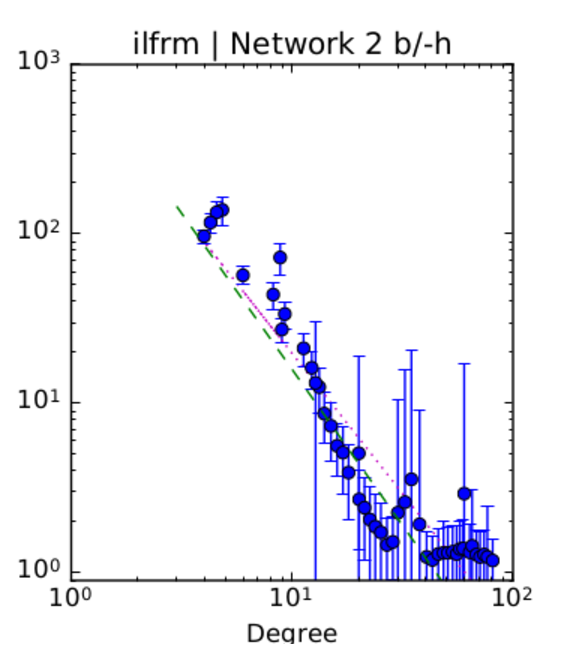
\includegraphics[scale=0.4]{\lpath/img/ilfrm_g2_d}
	\endminipage
	\minipage{0.25\textwidth}
	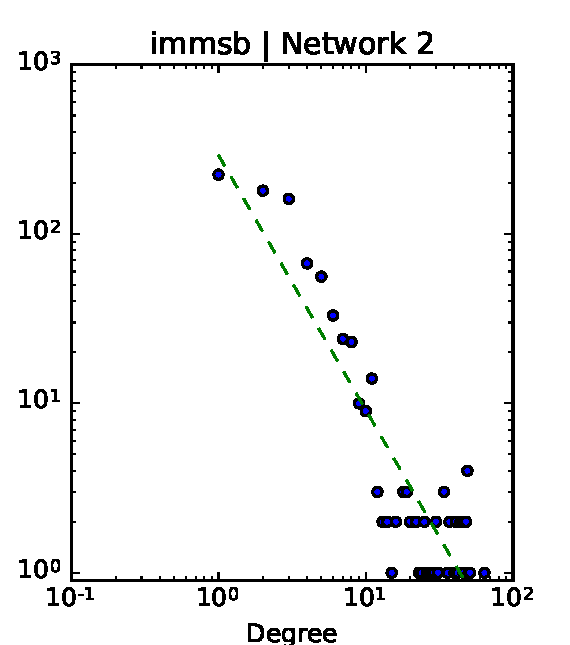
\includegraphics[scale=0.4]{\lpath/img/immsb_g2_d}
	\endminipage
	\vspace{-0.4cm}
	\minipage{0.25\textwidth}
	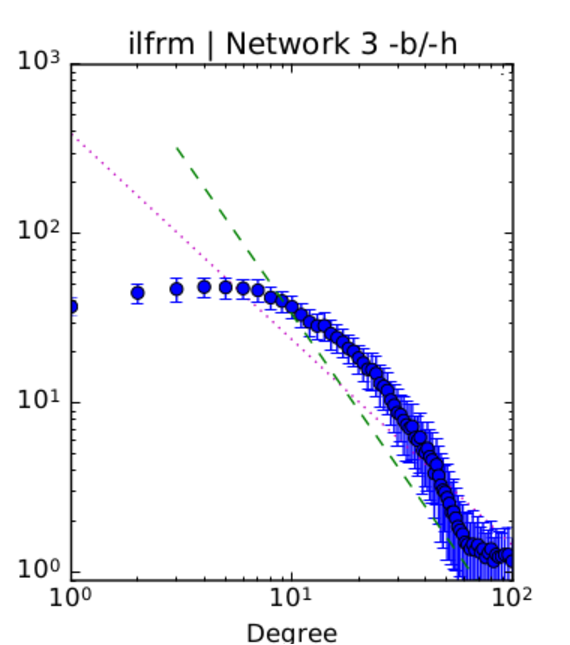
\includegraphics[scale=0.4]{\lpath/img/ilfrm_g3_d}
	\endminipage
	\minipage{0.25\textwidth}
	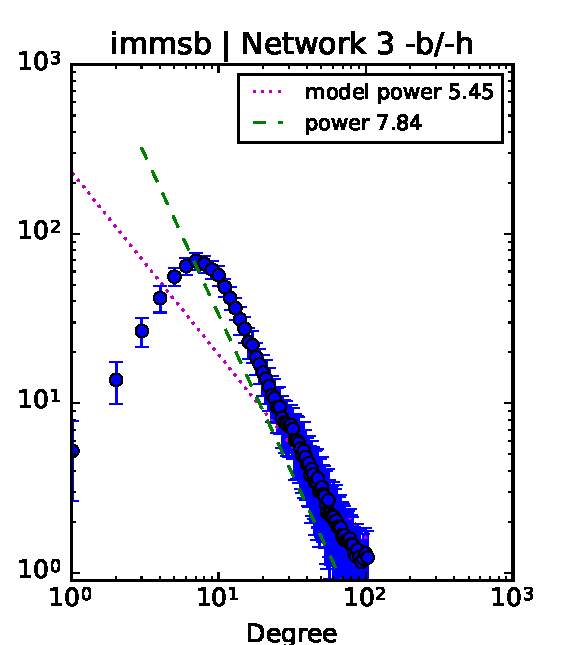
\includegraphics[scale=0.4]{\lpath/img/immsb_g3_d}
	\endminipage
	\vspace{-0.4cm}
	\minipage{0.25\textwidth}
	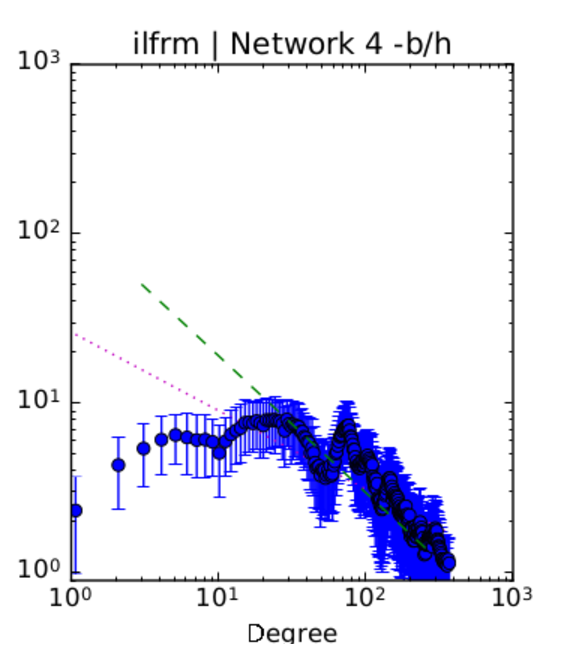
\includegraphics[scale=0.4]{\lpath/img/ilfrm_g4_d}
	\endminipage
	\minipage{0.25\textwidth}
	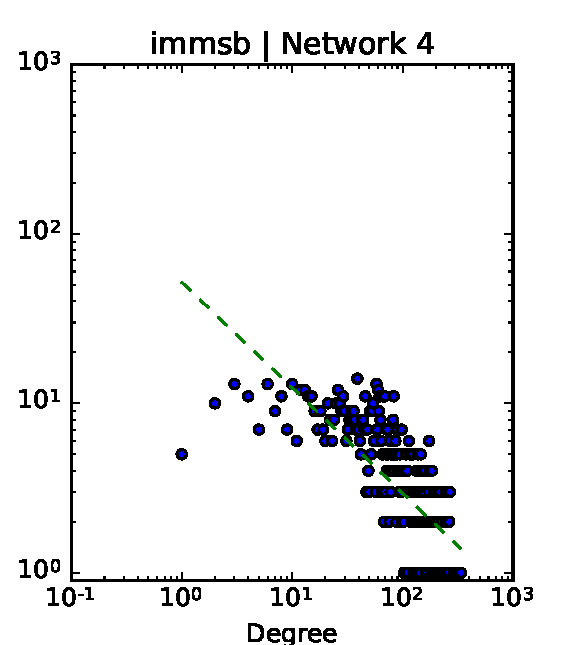
\includegraphics[scale=0.4]{\lpath/img/immsb_g4_d}
	\endminipage
	
	\caption{Right column is associated to IMMSB and left column to ILFM. Each row is associated to a synthetic networks on which we run the inference procedure. Each figures represent the global degrees distribution for a set of 100 generated networks by the models after its parameters where learned in the corresponding settings.  We also report on these figures two straight lines corresponding of the regression on the degree distribution of the model generated network (dotted) and the regression of the original distribution (dashed) as a qualitative reference.}
	\label{fig:gen_graph_s}
\end{figure}

\begin{figure}[h]
	\centering
	
	\minipage{0.25\textwidth}
	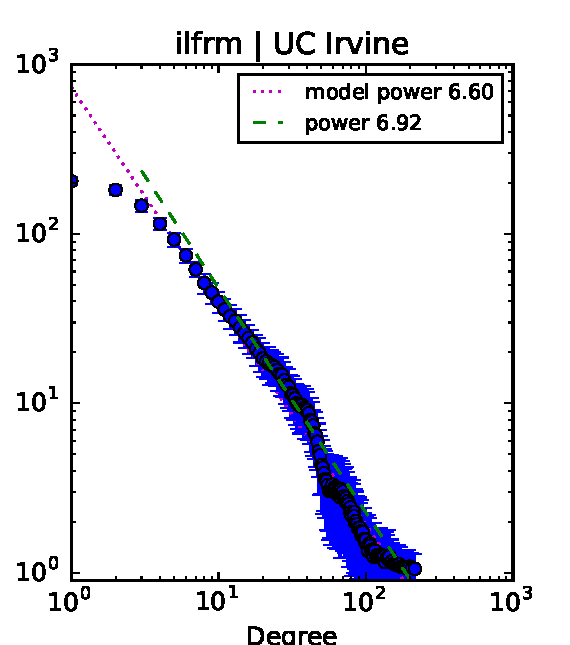
\includegraphics[scale=0.4]{\lpath/img/ilfrm_irvine_d}
	\endminipage
	\minipage{0.25\textwidth}
	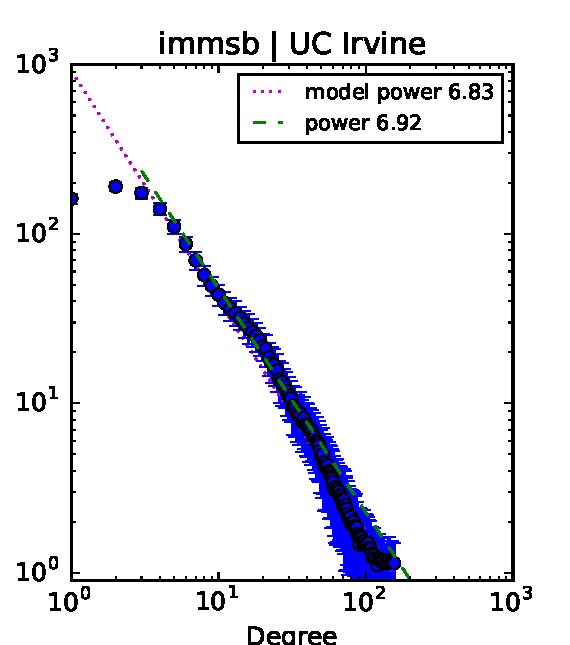
\includegraphics[scale=0.4]{\lpath/img/immsb_irvine_d}
	\endminipage
	\vspace{-0.4cm}
	\minipage{0.25\textwidth}
	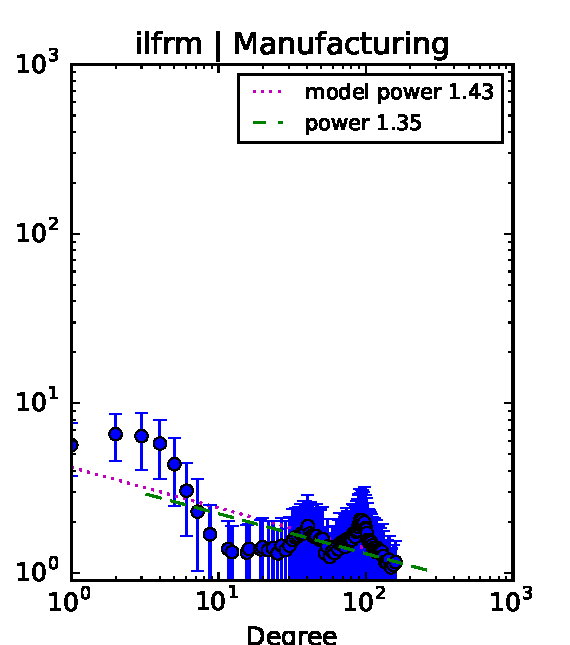
\includegraphics[scale=0.4]{\lpath/img/ilfrm_manufacturing_d}
	\endminipage
	\minipage{0.25\textwidth}
	\includegraphics[scale=0.4]{\lpath/img/immsb_manufacturing_d}
	\endminipage
	
	\caption{Right column is associated to IMMSB and left column to ILFM. Each row is associated to a real networks on which we run the inference procedure. Each figures represent the global degrees distribution for a set of 100 generated networks by the models after its parameters where learned in the corresponding settings. We also report on these figures two straight lines corresponding of the regression on the degree distribution of the model generated network (dotted) and the regression of the original distribution (dashed) as qualitative reference.}
	\label{fig:gen_graph_r}
\end{figure}


\begin{figure}[h]
	\centering
	
	\minipage{0.25\textwidth}
	\includegraphics[scale=0.22]{\lpath/img/M_e/AUC-ROC/figure_1}
	\endminipage
	\minipage{0.25\textwidth}
	\includegraphics[scale=0.22]{\lpath/img/M_e/AUC-ROC/figure_2}
	\endminipage
	\vspace{-0.4cm}
	\minipage{0.25\textwidth}
	\includegraphics[scale=0.22]{\lpath/img/M_e/AUC-ROC/figure_3}
	\endminipage
	\minipage{0.25\textwidth}
	\includegraphics[scale=0.22]{\lpath/img/M_e/AUC-ROC/figure_4}
	\endminipage
		\vspace{-0.4cm}
	\minipage{0.25\textwidth}
	\includegraphics[scale=0.22]{\lpath/img/M_e/AUC-ROC/figure_5}
	\endminipage
	\minipage{0.25\textwidth}
	\includegraphics[scale=0.22]{\lpath/img/M_e/AUC-ROC/figure_6}
	\endminipage
	
	\caption{AUC curves that compare the performance of ILFM and IMMSB on the 4 synthetic networks.}
	\label{fig:auc}
\end{figure}



\subsection{Results}

%%% Figure description:
We report in table \ref{table:unbalanced} our results for the prediction performance in the different settings. The prediction problem is equivalent to a binary prediction problem, where the prediction lies in two classes; edge or not an edge. The local precision and recall in the table concern the links predicted as an edge. The global (precision) refer to the accuracy of the model. The table summarize the precision and recall into the $f_1$ measure. Note that each group of row is indexed by  a number $K$ which indicates various values of initialization of the latent feature dimension.

Comparatively, in figure \ref{fig:auc}, we report the Area Under Curve for each datasets where we compare the prediction performance of IMMSB and ILFM on the task of links prediction.

In figure \ref{fig:gen_graph_s} and \ref{fig:gen_graph_r} we used the models learned on the training datasets to generate full networks and report the global degree distribution of such generated networks. 

%%% What the figure tells:
comparing the performance between both models in the links prediction precision and recall and $F_1$ measure (ref{table:unbalanced}), can seem to conflict with results in the ROC curve (\ref{fig:auc}). More precisely we see that ILFM dominate IMMSB on the $f_1$ measures on all experiments except for one (network 1, K=15). But on the AUC-ROC analysis( \ref{fig:auc}) we see that IMMSB dominate ILFM for two networks (Networks 1 and Networks 2), although it's number of latent feature is almost half lesser than for ILFM. This behavior is also reflected on the accuracy for both models (global precision); The accuracy of IMMSB models is higher for the Network1 and Network2, and this is the opposite for ILFM, which are more accurate for Network3 and Network4. Interestingly, we see that for ILFM, the dimension of the latent feature for which ILFM converged, for the two first networks is significantly higher than the two other. In other words the ILFM model seems to compensate is weak performance by increasing the number of features.

In the other hands, according to the degree distribution of the 4 synthetic networks we fitted, (figure \ref{fig:synt_graph}) and the p-value associated the power law hypothesis (table \ref{table:artificial_networks}), we see that the Network1 and Network2 has a stronger preferential attachment effects than Network3 and Network4.


Finally, the difference of behaviors of the models according to the training networks is captured by the randomness of the (generated) degree distributions (figure \ref{fig:gen_graph_s} ). We see that the degree distribution corresponding to the two bursty synthetic network, has  a high variance for ILFM while it is quite smooth for IMMSB.

The success of ILFM on bursty networks reflects the fact ILFM can handle the local preferential attachments and not ILFM. We assume that this symptom for ILFM is due to the hard assignment of it's latent features, where a difference of one feature, in a feature vector, can lead to a big gap in the probability to generate a link. A phenomenon particularly strong for very bursty networks where the long tail makes the distribution of degrees more sensitive to little change.

\textcolor{red}{Nothing about real networks: result are not really interesting except why ILFM variance of degree distribution on bursty networks fb\_uc is smooth ? }

To conclude, these experiments show that a properties based approach can help to choose an appropriate models. Moreover a model that seems to outperforms an other with a particular measure could be non optimal depending on what we want to capture in the data, keeping in mind that one measures is associated, in some way, to one behaviors or property.

\section{Related Work}

%Burstiness on topic model:
%Modeling Word Burstiness Using the Dirichlet Distribution (DCM)
%Accounting for Burstiness in Topic Models (DCMLDA)
%Proposal of a-MMSB in : Scalable Inference of Overlapping Communities with high diagonal only...

%to read: Stochastic blockmodels and community structure in networks

Recently, the MMSB \cite{MMSB} and ILFM \cite{ILFM} models have been successfully used for link predictions and structure discovery in social networks. Several extensions, has been proposed. In \cite{AMMSB}, they proposed a adaptation of a MMSB model that scale well using stochastic variational inference and use it for the discovery of overlapping communities in big networks (millions of nodes). They constrained the weight matrix to have weights in the diagonal and a fixed small value elsewhere and named it a-MMSB where "a" stand for assortative. The MMSB model has also been extended to a nonparametric dynamic version to handle temporal networks \cite{fan2015dynamic}. ILFM has also been extended in several way; to handle non-negative weights in \cite{IMRM} and within a more subtle latent feature structure in \cite{ILAM}. Nevertheless the characterization of models with regards to the properties for networks remains to be explored \cite{jacobs2014unified}. Theoretical results on the structure of random graph under exchangeability assumptions are however well reported in \cite{orbanz2015bayesian}, although the characterization of social networks properties within a Bayesian framework is not covered. In \cite{hoff2008modeling}, the role of exchangeability was first pointed out and its relation to the data representation where they provide a comparative study of the homophily and structural equivalence in different model settings, but without a formal definition of both. An other important mention of the exchangeability assumptions, was done in \cite{bickel2009nonparametric} where they characterize the asymptotic comportment of the likelihood in the blockmodel settings, showing that the inference of the likelihood lead to a consistent estimation of the community structure. But they only cover the case a single membership.


\section{Conclusion}
\label{sec:concl}

%%% Conclusion on the paper
This work introduce a framework which aims at studying topological properties on social networks by giving definitions which are consistent with the Bayesian framework. Using this framework, We show that strong relation between major relational latent model and fundamental properties of networks, particularly the preferential attachment effect and the homophily effect.~\\ 

%%% Perspectives
This work offers many perspectives to improve our understanding of Bayesian relational models for complex networks. Obviously, our implementation based on MCMC inference does not allow us to scale to large networks. We will focus in the future in implementing variational inference scheme to be able to conducts simulations on much larger real and synthetic networks. An other direction is to study the impact of hyperparameters on the structure of the generative network. Particularly a more well adapted optimization for nonparametric models could lead to a better control for capturing the preferential attachment effect. Especially by generalizing both the IBP and the HDP prior to their general counterpart, the 2-parameters IBP and the Pitman-Yor Process. To conclude on perspectives, it worth to mention that complex networks include other important properties of networks to study, such as the small world effect and the temporal dynamics of the network topology relaxing the exchangeability assumption.

\clearpage

\bibliographystyle{unsrt}
\bibliography{a}

\appendix
\section{Appendix}
\label{sec:append}

\subsection{Mixed membership Models}
\label{sec:mixmembership}
In the Mixed Membership Models \cite{MMM}, the models can be defined at the link level by the likelihood of generating a link between two nodes given the contribution of each classes (or features). For IMMSB, this likelihood is straightforward, but for ILFM the class membership is defined deterministically by the binary vector $\mat{f}$. If the $k^{th}$ row is active (equal to one) then the node has the membership, else it doesn't. Hence for ILFM, We can write the likelihood  using the Dirac distribution $\delta(x)$ that gives one for $x=0$ as follows:

\begin{align}
    \pr(y_{ij} \mid \mat{F}, \mat{\Phi } ) &= \sigma \sum_{k, k'} \pr(y_{ij}\mid\phi_{k,k'}) \pr(k \mid \mat{f}_i) \pr(k' \mid \mat{f}_j) \\
    &=  \sigma \sum_{k, k'} \phi_{k,k'}  \delta(1-f_{ik}) \delta(1-f_{jk'})
    \end{align}
    

\subsection{Collapsed Gibbs sampling updates for IMMSB}

We provide here the derivation of the updates of the IMMSB model, described in Section~\ref{sec:models}.

%From the definition of the model, one has: $\pr(z_{ij} = k \mid \mat{f}_i) = f_{ik}$.

%\textcolor{red}{Adrien, peux-tu donner la d\'erivation ? La forme actuelle n'est valable que pour MMSB.} 

%heeeere \alpha is \alpha_0

Inference for the IMMSB model by using the Collapse Gibbs sampler gives updates for class assignment $Z \in N\times N \times 2$ for each interactions $Y \in N\times N$. Thus for all pair of interaction (i,j) we jointly sample the classes $(z_{ij}, z_{ji})$ who implicitly, take the values $(k,k')$ :
\begin{align} \label{eq:cgs}
&\pr(z_{ij}, z_{ji} \mid Z^-, Y,  \mat{\beta}, \alpha, \mat{\lambda} )  \\
&\propto\pr(z_{ij}, z_{ji} \mid Z^-, \alpha,\mat{\beta}) \pr(y_{ij} \mid Y^{-ij},  Z^-,z_{ij}, z_{ji},  \mat{\lambda} ) \nonumber
\end{align}
The term $Z^-$ denote that both $z_{ij}$ and $z_{ji}$ are exclude from $Z$. We now treat the first term of equation \ref{eq:cgs}.  
\begin{align}
&\pr(z_{ij}, z_{ji} \mid Z^-, \alpha,\mat{\beta})\\
&\propto \pr(z_{i\rightarrow j} \mid \{z_{i\rightarrow j'}\}_{j'\neq j}, \{z_{j'\leftarrow i}\}_{j'=1}^N, \alpha,\mat{\beta}) \\
& \quad .  \pr(z_{i\leftarrow j} \mid \{z_{i'\leftarrow j}\}_{i'\neq i}, \{z_{j\leftarrow i'}\}_{i'=1}^N, \alpha,\mat{\beta}) \nonumber
\end{align}
Let's consider the density of $z_{i\rightarrow j}$:
\begin{align}
&\propto \pr(z_{i\rightarrow j} \mid \{z_{i\rightarrow j'}\}_{j'\neq j}, \{z_{j'\leftarrow i}\}_{j'=1}^N, \alpha,\mat{\beta})  \\
&\propto \int_{f_i} \pr(f_i \mid \mat{\beta}, \alpha) \pr(z_{ij} \mid f_i) \prod_{j'\neq j} \pr(z_{ij'} \mid f_i) \prod_{j' =  1}^N  \pr(z_{j' i} \mid f_i)  df_i \nonumber
\end{align}


Due to the an augmented representation of the Chinese Restaurant Franchise (CRF) with the Stick Breaking Process \cite{HDP}, the density of the features can be approximated by the following Dirichlet distribution;
\begin{equation}
f_i \mid \mat{\beta}, \alpha \sim Dir(\alpha \beta_1,..,\alpha\beta_K, \alpha\beta_{new})
\end{equation}
Where $\alpha\beta_{new}$ represent the contribution for sampling a new class. Since $\pr(z_{ij} \mid f_i)$ is drawn from a multinomial, the model is said to be conjugate and reduce to a simple closed form expression:
\begin{enumerate}
\item If the class $k$ has already been observed:
   \begin{align}
    \pr(z_{ij} =k \mid .) &\propto N_{ik}^{-ij} + \alpha_0 \beta_k
    \label{eq:update-immsb}
   \end{align}
\item In case of a new class $k_{new}$:
   \begin{align}
    \pr(z_{ij} =k_{new} \mid.) &\propto \alpha_0 \beta_{new} \nonumber   
   \end{align}
\end{enumerate}
 Where  $N_{ik}$ is the count for node $i$ being assigned to class $k$. As we show that the equations are symmetric, sampling for $z_{ji}$ is straightforward.

~\\
Again, referring the CRF, the sampling of the tables configuration $\mat{m}$ is given by: 
\begin{equation}
\pr(m_{ik} \mid Z, \bm{m}^{-ik}, \mat{\beta} ) = \frac{\Gamma(\alpha_0 \beta_k)}{\Gamma(\alpha_0 \beta_k + n_{j\bm{.   }k})} s(n_{j\bm{.}k}, m) (\alpha_0 \beta_k)^m
\end{equation}
And, finnaly  $\mat{\beta}$ is obtained by:
\begin{equation}
\mat{\beta} \sim Dir(m_1,.., m_K, \gamma)  
\end{equation}
Where $s(n,m)$ is the unsigned Stirling number of the first kind.


~\\
Finally, when the markov chain reach the stationnary distribution, the models parameters $\M = \{\mat{\Phi}, \mat{F}\}$ can be recovered by averaging the topics assignement counts for each membership and each relation:
\begin{align}
&\hat f_{ik} =\frac{ N_{ik} + \alpha\beta_k}{ N + \sum_k\alpha_k }\\
&\hat \phi_c  = \frac{M_{c1} + \lambda_1}{M_{c\bm{.}} + \lambda_0 + \lambda_1}
\end{align}


The count for node $i$ being assigned to membership $k$ is $N_{ik}$. And the count of for all couple of classes $c=(k,k')$ being associated to relation $r$ is $M_{cr}$. Note that in our case, the relation $r$ take values in (0,1) accounting for link or non-link between two node.

\section{Precision Recall Results}
\label{sec:precision_recall}

% Debug 12 / MASK all

% K = 5

\begin{table*}[h] \label{table:unbalanced}
\caption{Predictive Performance on a UnBalanced Testing set}
	\begin{minipage}[h]{0.45\linewidth} 
K = 5\hspace{5pt}
\begin{tabular}{lllll}
\hline
 IMMSB   &   global &   precision &   recall &    K-\ensuremath{>} \\
\hline
 Network1 b/h         &    0.990 &       0.029 &    0.032 & 5.0 $\pm$ 0.0 \\
 Network2 b/-h       &    0.992 &       0.032 &    0.034 & 5.0 $\pm$ 0.0 \\
 Network3 -b/h       &    0.979 &       0.031 &    0.034 & 5.0 $\pm$ 0.0 \\
 Network4 -b/-h       &    0.887 &       0.151 &    0.192 & 5.0 $\pm$ 0.0 \\

\hline
\end{tabular}
\end{minipage}
\hspace{0.8cm}
\begin{minipage}[h]{0.45\linewidth}
\begin{tabular}{lllll}
\hline
  ILFRM & global &   precision &   recall &     K-\ensuremath{>} \\
\hline
 Network1 b/h       &    0.990 &       0.051 &    0.053 & 13.4 $\pm$ 0.8    \\
 Network2 b/-h     &    0.992 &       0.044 &    0.045 & 14.0 $\pm$ 2.0    \\
 Network3 -b/h     &    0.982 &       0.114 &    0.116 & 10.0 $\pm$ 2.1 \\
 Network4 -b/-h     &    0.926 &       0.389 &    0.393 & 7.2 $\pm$ 1.6     \\

\hline
\end{tabular}
\end{minipage}

% K = 10

	\begin{minipage}[h]{0.45\linewidth} 
K = 10
\begin{tabular}{lllll}
Network1 b/h         &    0.990 &       0.044 &    0.046 & 10.0 $\pm$ 0.0 \\
 Network2 b/-h       &    0.992 &       0.039 &    0.045 & 10.0 $\pm$ 0.0 \\
 Network3 -b/h       &    0.979 &       0.030 &    0.035 & 10.0 $\pm$ 0.0 \\
 Network4 -b/-h       &    0.897 &       0.202 &    0.238 & 10.0 $\pm$ 0.0 \\

\hline
\end{tabular}
\end{minipage}
\hspace{0.8cm}
\begin{minipage}[h]{0.45\linewidth}
\begin{tabular}{lllll}
 Network1 b/h       &    0.990 &       0.049 &    0.053 & 17.2 $\pm$ 2.8 \\
 Network2 b/-h     &    0.992 &       0.047 &    0.051 & 17.2 $\pm$ 2.1 \\
 Network3 -b/h     &    0.982 &       0.132 &    0.132 & 12.2 $\pm$ 2.0 \\
 Network4 -b/-h     &    0.934 &       0.448 &    0.447 & 9.2 $\pm$ 1.2 \\

\hline
\end{tabular}
\end{minipage}

% K = 15

	\begin{minipage}[h]{0.45\linewidth} 
K = 15
\begin{tabular}{lrrrr}
 Network1 b/h         &    0.990 &       0.038 &    0.041 & 15.0 $\pm$ 0.0 \\
 Network2 b/-h       &    0.992 &       0.036 &    0.038 & 15.0 $\pm$ 0.0 \\
 Network3 -b/h       &    0.979 &       0.029 &    0.032 & 15.0 $\pm$ 0.0 \\
 Network4 -b/-h       &    0.898 &       0.207 &    0.245 & 15.0 $\pm$ 0.0 \\

\hline
\end{tabular}
\end{minipage}
\hspace{0.8cm}
\begin{minipage}[h]{0.45\linewidth}
\begin{tabular}{lrrrr}
 Network1 b/h       &    0.990 &       0.050 &    0.053 & 20.6 $\pm$ 2.1 \\
 Network2 b/-h     &    0.992 &       0.049 &    0.055 & 21.2 $\pm$ 2.1 \\
 Network3 -b/h     &    0.983 &       0.164 &    0.166 & 17.2 $\pm$ 1.3 \\
 Network4 -b/-h     &    0.939 &       0.499 &    0.501 & 14.8 $\pm$ 0.4    \\

\hline
\end{tabular}
\end{minipage}

% K = 20

	\begin{minipage}[h]{0.45\linewidth} 
K = 20
\begin{tabular}{lrrrr}

 Network1 b/h          &   0.9899 &      0.0348 &   0.0375 & 20 \\
 Network2 b/-h       &   0.9923 &      0.0494 &   0.0590 & 20 \\
 Network3 -b/-h      &   0.9794 &      0.0289 &   0.0338 & 20 \\
 Network4 -b/h        &   0.9067 &      0.2646 &   0.3034 & 20 \\
\hline
\end{tabular}
\end{minipage}
\hspace{0.8cm}
\begin{minipage}[h]{0.45\linewidth}
\begin{tabular}{lrrrr}
Network1 b/h       &   0.9902 &      0.0641 &   0.0626 &  23 \\
Network2 b/-h     &   0.9915 &      0.0477 &   0.0636 & 17 \\
Network3 -b/h     &   0.9827 &      0.1523 &   0.1518 &  20 \\
Network4 -b/-h     &   0.9396 &      0.4986 &   0.5053 &  22 \\
\hline
\end{tabular}
\end{minipage}
\end{table*}


%%%%%%%%%%%%%%%%%%%%%%%%%%%%%%%%%%%%%%%%%%%%%%%%%%%%%%%%%%%%%%%%%%%%
%%%%%%%%%%%%%%%%%%%%%%%%%%%%%%%%%%%%%%%%%%%%%%%%%%%%%%%%%%%%%%%%%%%%
%%%%%%%%%%%%%%%%%%%%%%%%%%%%%%%%%%%%%%%%%%%%%%%%%%%%%%%%%%%%%%%%%%%%
%%%%%%%%%%%%%%%%%%%%%%%%%%%%%%%%%%%%%%%%%%%%%%%%%%%%%%%%%%%%%%%%%%%%
%%%%%%%%%%%%%%%%%%%%%%%%%%%%%%%%%%%%%%%%%%%%%%%%%%%%%%%%%%%%%%%%%%%%
%%%%%%%%%%%%%%%%%%%%%%%%%%%%%%%%%%%%%%%%%%%%%%%%%%%%%%%%%%%%%%%%%%%%


% Debug 11 / MASK 1

% K = 5

\begin{table*}[h] \label{table:balanced}
\caption{Predictive Performance on a Balanced Testing set}
	\begin{minipage}[h]{0.45\linewidth} 
K =  5\hspace{5pt}
\begin{tabular}{lrlll}
\hline
 IMMSB   &   global &   precision &   recall &    K-\ensuremath{>} \\
\hline
 Network1 b/h          &    0.549 &       0.758 &    0.022 & 5.0 $\pm$ 0.0 \\
 Network2 b/-h        &    0.558 &       0.834 &    0.019 & 5.0 $\pm$ 0.0 \\
 Network3 -b/h        &    0.527 &       0.729 &    0.027 & 5.0 $\pm$ 0.0 \\
 Network4 -b/-h        &    0.557 &       0.743 &    0.162 & 5.0 $\pm$ 0.0 \\

\hline
\end{tabular}
\end{minipage}
\hspace{0.8cm}
\begin{minipage}[h]{0.45\linewidth}
\begin{tabular}{lrlll}
\hline
 ILFRM   &   global &   precision &   recall &     K-\ensuremath{>} \\
\hline
 Network1 b/h        &    0.568 &       0.912 &    0.047 & 13.6 $\pm$ 2.3 \\
 Network2 b/-h      &    0.574 &       0.893 &    0.041 & 16.4 $\pm$ 3.4 \\
 Network3 -b/h      &    0.571 &       0.912 &    0.100 & 9.2 $\pm$ 1.3 \\
 Network4 -b/-h      &    0.668 &       0.906 &    0.362 & 7.6 $\pm$ 1.3 \\

\hline
\end{tabular}
\end{minipage}

% K = 10

	\begin{minipage}[h]{0.45\linewidth} 
K = 10
\begin{tabular}{lrrrr}
 Network1 b/h          &    0.558 &       0.842 &    0.028 & 10.0 $\pm$ 0.0 \\
 Network2 b/-h        &    0.567 &       0.926 &    0.034 & 10.0 $\pm$ 0.0 \\
 Network3 -b/h        &    0.530 &       0.776 &    0.027 & 10.0 $\pm$ 0.0 \\
 Network4 -b/-h        &    0.567 &       0.764 &    0.184 & 10.0 $\pm$ 0.0 \\

\hline
\end{tabular}
\end{minipage}
\hspace{0.8cm}
\begin{minipage}[h]{0.45\linewidth}
\begin{tabular}{lrrrr}
 Network1 b/h        &    0.556 &       0.928 &    0.044 & 17.2 $\pm$ 2.0 \\
 Network2 b/-h      &    0.573 &       0.935 &    0.041 & 17.6 $\pm$ 3.2    \\
 Network3 -b/h      &    0.579 &       0.947 &    0.118 & 12.8 $\pm$ 0.9 \\
 Network4 -b/-h      &    0.718 &       0.943 &    0.457 & 10.8 $\pm$ 0.7 \\

\hline
\end{tabular}
\end{minipage}

% K = 15

	\begin{minipage}[h]{0.45\linewidth} 
K = 15
\begin{tabular}{lrrrr}
 Network1 b/h          &    0.555 &       0.871 &    0.035 & 15.0 $\pm$ 0.0 \\
 Network2 b/-h        &    0.570 &       0.854 &    0.030 & 15.0 $\pm$ 0.0 \\
 Network3 -b/h        &    0.532 &       0.728 &    0.027 & 15.0 $\pm$ 0.0 \\
 Network4 -b/-h        &    0.565 &       0.757 &    0.178 & 15.0 $\pm$ 0.0 \\

\hline
\end{tabular}
\end{minipage}
\hspace{0.8cm}
\begin{minipage}[h]{0.45\linewidth}
\begin{tabular}{lrrrr}
 Network1 b/h        &    0.569 &       0.928 &    0.046 & 20.8 $\pm$ 1.3 \\
 Network2 b/-h      &    0.564 &       0.903 &    0.042 & 21.6 $\pm$ 2.4 \\
 Network3 -b/h      &    0.594 &       0.952 &    0.153 & 18.0 $\pm$ 0.8 \\
 Network4 -b/-h      &    0.723 &       0.945 &    0.467 & 15.0 $\pm$ 0.0    \\

\hline
\end{tabular}
\end{minipage}

% K = 20

	\begin{minipage}[h]{0.45\linewidth} 
K = 20
\begin{tabular}{lrrrr}

 Network1 b/h           &   0.5501 &      0.8980 &   0.0425 & 20 \\
 Network2 b/-h        &   0.5734 &      0.9615 &   0.0326 & 20 \\
 Network3 -b/-h       &   0.5286 &      0.6456 &   0.0255 & 20 \\
 Network4 -b/h         &   0.5577 &      0.7475 &   0.1662 & 20 \\
\hline
\end{tabular}
\end{minipage}
\hspace{0.8cm}
\begin{minipage}[h]{0.45\linewidth}
\begin{tabular}{lrrrr}
 Network1 b/h         &   0.5428 &      0.9737 &   0.0359 &  21 \\
 Network2 b/-h      &   0.5577 &      0.8462 &   0.0389 &  20 \\
 Network3 -b/-h     &   0.5997 &      0.9503 &   0.1630 &  22 \\
 Network4 -b/-h      &   0.7291 &      0.9473 &   0.4813 & 20 \\
\hline
\end{tabular}
\end{minipage}
\end{table*}




\end{document}

\grid
